%!TEX root = ../thesis.tex

\chapter{High-level triggers for Top Physics}
\label{c:service_work}
\ifpdf
    \graphicspath{{04_Service_work/plots/}}
\else
    \graphicspath{{04_Service_work/plots/EPS/}{04_Service_work/plots/}}
\fi

The LHC is often referred to as a top quark factory, producing a \ttbar pair nearly each second of its nominal
operation. While the production rate of \SI{\approx1}{\Hz} seems manageable in terms of recording the data, it is
significantly complicated by background processes with similar signatures occurring at much higher rates.

The trigger is the starting point of any physics event selection process, and therefore is clearly important for any
physics analysis. As mentioned in Section~\ref{ss:trigger_daq}, the CMS L1 trigger rate is limited to
\SI{\sim100}{\kilo\hertz}. In order to meet the data recording constraints of approximately
\SI{300}{\mega\byte\per\second}, this rate is further reduced down to \SI{\sim300}{\Hz}, which is done by the HLT
system. The total rate budget has to be allocated to maximise the acceptance across the full range of the CMS physics
programme, which can be a matter of serious debate.

During the LHC operation in 2011 and 2012 under conditions of gradual increase of instantaneous luminosity and pile-up,
but very limited rate budget, trigger developers constantly tackled the challenge of finding the best compromise between
growing rates and maintaining reasonable signal acceptance. While the simplest approach is tightening the cuts on
physical quantities like lepton or jet transverse momenta, it is not favourable since it lowers the number of stored
signal events and decreases the phase space which is crucial for new physics searches as well as Standard Model
precision measurements. Therefore, the development of more efficient algorithms is the most preferable solution,
allowing a high level of acceptance to be kept for signal events, whilst effectively rejecting background events. This
can often be achieved by reducing the level of approximation of the online (HLT) object reconstruction, making the
algorithms closer to their sophisticated offline counterparts. However, it leads to a higher execution time, which is
limited by computing resources available for HLT reconstruction. Hence, the CPU timing is another major constraint faced
by the HLT developers.

This chapter covers the author's contribution to development and verification of High-Level Triggers for top physics
with a semileptonic signature, where one of the W bosons decays into an electron and a neutrino. The description of top
triggers, efficiency measurement, validation of jet energy corrections and pile-up subtraction applied at the HLT level
are discussed in relevant sections of this chapter.

\section{Level-1 triggers}
The CMS L1 trigger \autocite{CMS_L1_Trigger_TDR} is built of custom electronics processing the data from the
calorimeters and the muon system. It is the first filtering stage of any physics selection, therefore it has high
requirements on efficiency and phase space acceptance. The input rate of events, i.e.\ the beam crossing frequency of
\SI{\sim5e8}{\hertz} must be reduced down to \SI{\sim100}{\kilo\hertz}. This represents a major challenge considering a
gradual increase of instantaneous luminosity throughout the LHC operation. The rate budget of \SI{\sim100}{\kilo\hertz}
is shared between several L1 triggers corresponding to different physics objects being present in the event. For top
physics signatures with a single electron in the final state, the following triggers have been used:

\begin{itemize}
 \item L1\_SingleEG\_18
 \item L1\_SingleEG\_20
 \item L1\_SingleEG\_22
\end{itemize}

These triggers are referred to as electron/photon (e/$\gamma$, or EG) triggers. They scan the ECAL for groups of trigger
cells\footnote{Each trigger cell is formed by $5 \times 5$ crystals in the barrel region, corresponding to dimensions of
$\Delta\eta \times \Delta\phi = \num{0.087 x 0.087}$; these numbers vary in the endcap region
\autocite{CMS_L1_Trigger_TDR}.} ($4 \times 4$) with a summed energy above the threshold that is suggested by the name of
the trigger (\SIlist{18;20;22}{\GeV}). The choice of threshold is determined by sustainability of the trigger rate at a
given instantaneous luminosity.

\begin{figure}[!htbp]
  \centering
  \leavevmode
  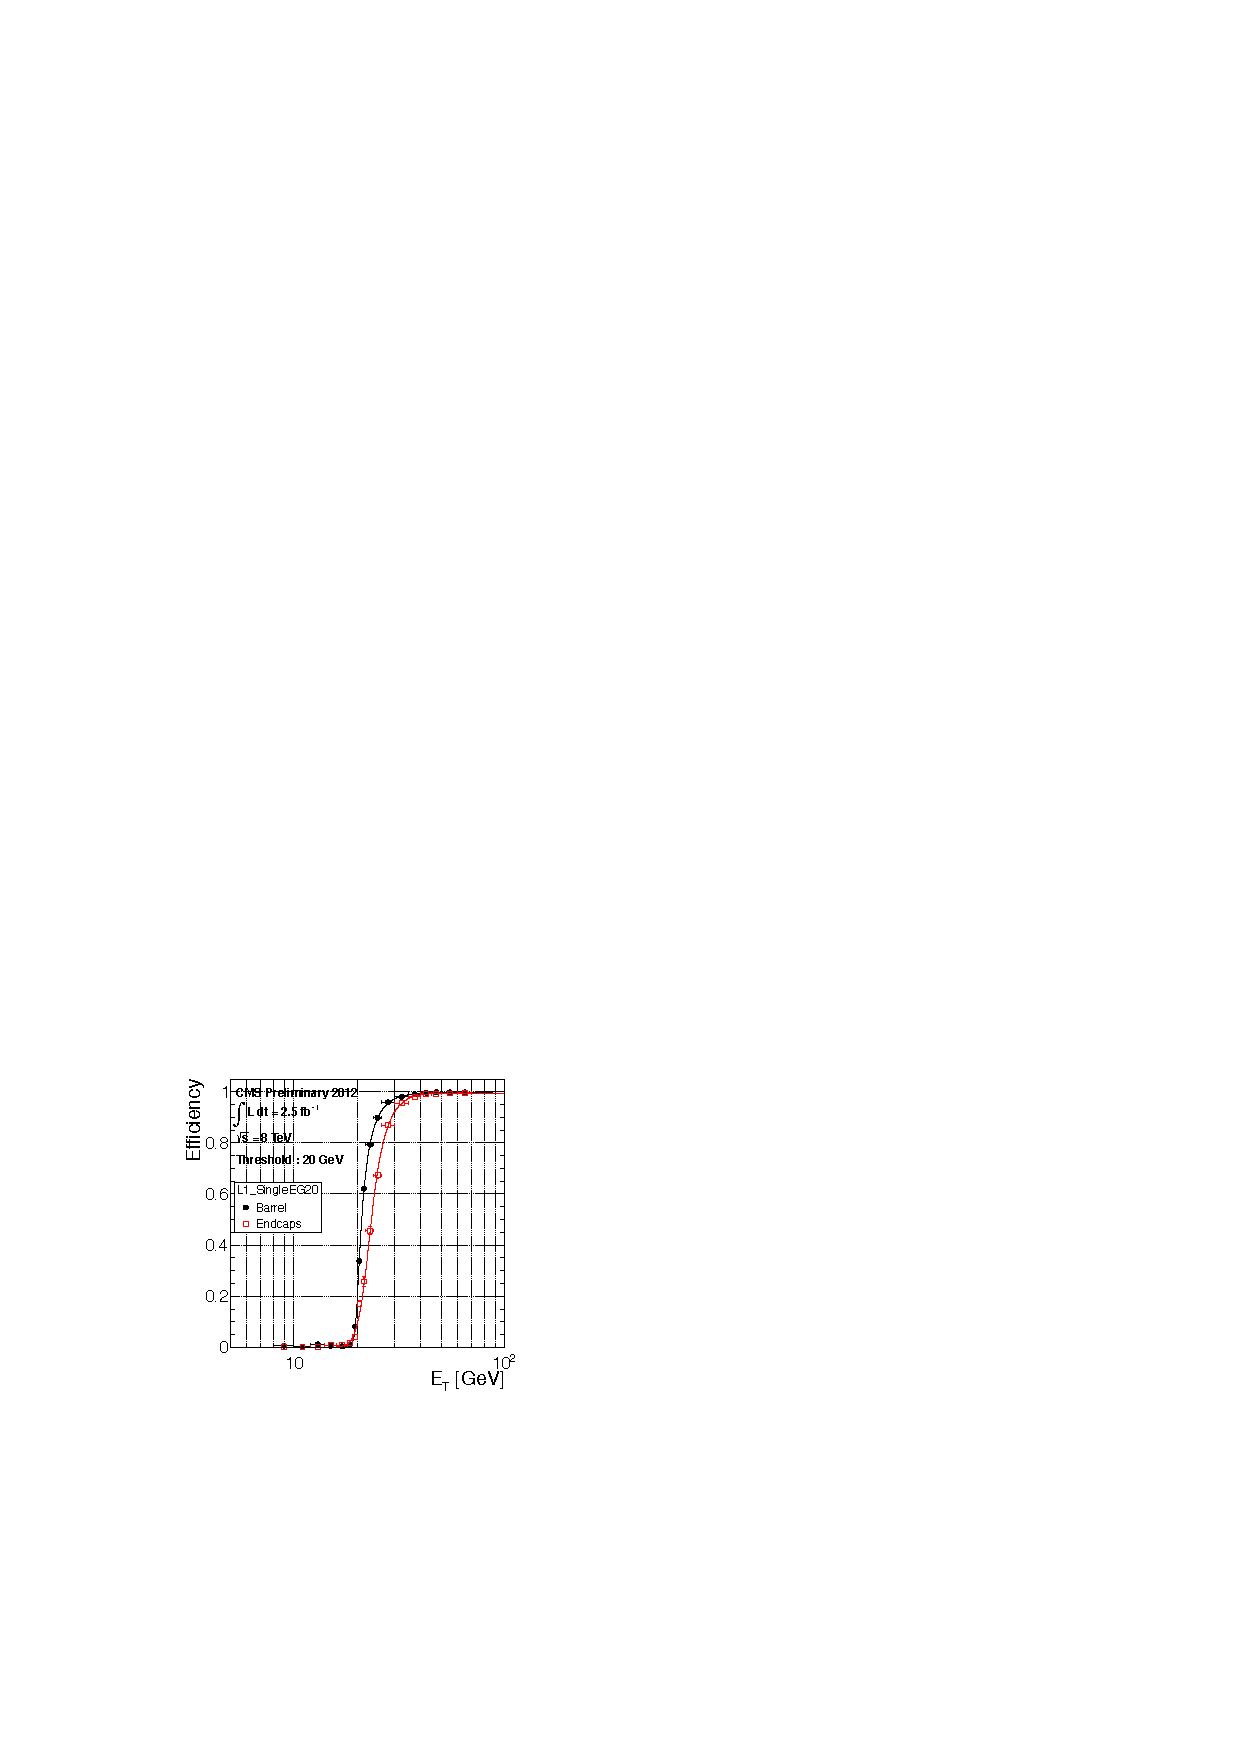
\includegraphics[width=0.5\columnwidth]{L1_turnon}
  \caption[Efficiency of the \SI{20}{\GeV} e/$\gamma$ trigger]{Efficiency of the \SI{20}{\GeV} e/$\gamma$ trigger as a
  function of offline \ET, shown separately for barrel and endcap regions \autocite{L1_Brooke}.}
  \label{fig:L1_seed_turn_on_curve}
\end{figure}

The efficiency of the L1\_SingleEG\_20 trigger as a function of the electron transverse momentum reconstructed offline
is shown in Figure~\ref{fig:L1_seed_turn_on_curve}. Clearly, the turn-on curve of the trigger is sharper in the barrel
region than in the endcap region. The plateau region of the curve (\SI{\approx95}{\pc} efficiency) is reached at
\SI{\approx30}{\GeV} in the barrel and \SI{\approx35}{\GeV} in the endcap region. This difference in trigger efficiency
needs to be taken into account in the construction of the high-level trigger, as the L1 trigger decisions are used as
input ``seeds'' to the HLT system, which is described in the following section.

\section{High-level triggers for top physics}
\label{s:hlt_for_top_physics}
The High-Level Trigger \autocite{HLT} is the crucial part of CMS event selection process. As mentioned in
Section~\ref{ss:trigger_daq}, it is based on software algorithms running on the Event Filter Farm, i.e.\ a large cluster
of commercial CPUs. The HLT reconstruction, often referred to as online reconstruction, is implemented in the same
software framework (CMSSW) which is used for offline reconstruction, and the algorithms can be very similar. However,
the key difference between online and offline reconstruction is the running time. Since the HLT selection has to be
performed in real time, it imposes a significant constraint on computing resources, enforcing compromises on the
robustness and efficiency of online algorithms. With an exception of small samples for performance monitoring, data
rejected by the HLT is lost irrevocably. Therefore, correct and efficient operation of the HLT is of major importance
for the CMS physics programme.

The modular structure of CMSSW provides high flexibility in use of selection and reconstruction algorithms, allowing
their continuous optimisation according to changes in physics needs and data-taking conditions. Various modules account
for reconstruction of different physics objects and their matching with L1 objects, filtering, logging, monitoring, etc.
All these modules are grouped into so-called trigger ``paths'', ultimately giving trigger decisions on whether to accept
an event or not. A typical example of a trigger path used for top physics is an electron plus jets trigger, which
requires the presence of isolated electron and at least three energetic jets in the event.

A trigger path can be prescaled or unprescaled. Prescaling is a method of reducing the trigger rate by only recording a
fraction of events that pass the trigger selection. For example, if the prescale value of a particular trigger is 10,
only one out of ten events that fire the trigger will be actually recorded. Usually prescaled triggers are used for
performance monitoring and background estimation as they can impose a much looser selection criteria yet still have
manageable rate. However, such triggers are unfavourable for signal selection, as they greatly reduce signal acceptance.

A set of trigger paths and their prescale factors is combined in the HLT configuration, referred to as the HLT menu or
table \autocite{HLT_commissioning}. Since the start of data-taking in 2010, the CMS trigger coordination adopted a
``trigger train'' model, implying the schedule of regular deadlines for updates in the trigger menu. These deadlines are
usually imposed fortnightly, according to changes in instantaneous luminosity or other alterations in data-taking
conditions. In order for a trigger path to be included in the trigger menu, it has to be implemented in the HLT
configurations database, validated by measuring the trigger rate and signal efficiency, tested for CPU timing and
finally approved by the trigger studies group.

As mentioned before, the top quark pair decay covered in this work has a semileptonic signature, containing an electron,
at least four jets and a neutrino giving rise to \MET. Due to the nature of the decay, all these objects are highly
energetic and can be triggered on with rather high thresholds on transverse energy. During the start-up year of 2010
when the instantaneous luminosity went up from \SI{\sim e27}{\cm^{-2}~s^{-1}} to \SI{\sim e31}{\cm^{-2}~s^{-1}}, top
analyses with the signature of interest used the single electron trigger, requiring just one electron with certain
isolation and transverse momentum criteria. However, by extrapolating the trigger rates on higher luminosities foreseen
in the following years it became obvious that the single electron trigger rate would quickly become too high for the
rate budget restrictions at the time. Therefore, alternative ways of adding other objects from the \ttbar signature were
explored, naturally leading to electron plus jets trigger solution.

A typical electron plus jets trigger consists of a standard electron module, a jet module, a cleaning module to remove
overlap between jet and electron collections, and a jet multiplicity filter. The electron module is constructed from the
following sub-modules:

\begin{enumerate}
  \item L1 object and ECAL super-cluster matching;
  \item ECAL transverse energy filter;
  \item ECAL electron ID and isolation filter;
  \item HCAL electron ID and isolation filter;
  \item Tracker electron ID and isolation filter.
\end{enumerate}

To minimise the total running time, all the sub-modules are ordered by speed, starting from the fastest. The matching
module (1) finds the ECAL super-cluster closest to the L1 object in $\eta$ and $\phi$ dimensions. If the super-cluster is
located within a certain $\eta$ and $\phi$ range, the event is passed to the next module, otherwise it is rejected. The
following ECAL module (2) calculates the super-cluster transverse energy ($E_\mathrm{T}$), and as long as it is above
\SI{25}{\GeV}, the electron ID and isolation criteria are imposed using ECAL (3), HCAL (4) and the tracker (5)
information (see Section~\ref{ss:electron_reconstruction}).

The working points for identification and isolation criteria and their naming conventions are shown in
Table~\ref{tab:trigger_naming}. Working points studied for 2011 analysis (Chapter~\ref{c:top_mass_analysis}) were known
by the following descriptive labels: VeryLoose (VL), Loose (L), Tight (T), and VeryTight (VT). In 2012, the working
point known as WP80 was introduced for the use in single electron trigger, described later on.

\begin{table}[!hbp] \centering
\resizebox{\textwidth}{!}{
\begin{tabular}{lcccc}
\textbf{Working point} & \textbf{CaloID}  & \textbf{CaloIso} & \textbf{TrkId} & \textbf{TrkIso} \\
\hline
VeryLoose (VL) & $H/E <$ 0.15 (0.10) &  $\text{ECAL iso}/\ET<$ 0.2 (0.2) & $\Delta\eta <$ 0.01 (0.01) & $\text{track iso}/\pt<$ 0.2 (0.2)\\
 & $\sigma_{i\eta i\eta} <$ 0.024 (0.040) & $\text{HCAL iso}/\ET<$ 0.2 (0.2) & $\Delta\phi <$ 0.15 (0.10) & \\
 Loose (L) & $H/E <$ 0.15 (0.10) & &  & \\
 & $\sigma_{i\eta i\eta} <$ 0.014 (0.035) & &  & \\
 Tight (T) & $H/E <$ 0.10 (0.075) &  $\text{ECAL iso}/\ET<$ 0.125 (0.075) & $\Delta\eta <$ 0.008 (0.008) & $\text{track iso}/\pt<$ 0.125 (0.125)\\
 & $\sigma_{i\eta i\eta} <$ 0.011 (0.031) & $\text{HCAL iso}/\ET<$ 0.125 (0.125) & $\Delta\phi <$ 0.07 (0.05) & \\
 VeryTight (VT) & $H/E <$ 0.05 (0.05) &   & & \\
 & $\sigma_{i\eta i\eta} <$ 0.011 (0.031) &  &  & \\
 %TighterEleId  & $H/E <$ 0.05 (0.05) &  & $\Delta\eta <$ 0.008 (0.007) &\\
 %& $\sigma_{i\eta i\eta} <$ 0.011 (0.031) &  & $\Delta\phi <$ 0.10 (0.10) & \\
\hline
\end{tabular}
}
\caption[Naming conventions for electron trigger working points.]{Naming conventions for electron trigger working
points. The given values are for the barrel region of the detector and the values in brackets for the endcap region.}
\label{tab:trigger_naming} 
\end{table}
% source: https://twiki.cern.ch/twiki/bin/view/CMS/EgammaWorkingPointsv3 (restricted access so no reference)

In the main trigger path used for signal rather than background estimation in 2011 analysis, the Very Tight (VT) working
point for calorimeter identification (CaloID) and the Tight (T) working point for calorimeter isolation (CaloIso) were
used. This was motivated by consistency with similar criteria for the single electron trigger used in 2010.

For the events that pass all described criteria in the electron module, a simplified algorithm for offline iterative
tracking is applied. This algorithm has a faster running time at the expense of worse resolution. In order to decrease
the CPU usage, the Combinatorial Track Finder (CTF) \autocite{CTF_tracking} is used instead of the GSF one, and the
tracking is confined to a small region around the electron. The events are required to pass the tight criteria of the
tracker electron ID (TrkId) which is calculated at this stage. Finally, the tight working point of the tracker isolation
(TrkIso) is applied, where the track \pt is summed over all tracks within $\Delta R = 0.3$ cone around the electron
track, excluding the electron itself.

Provided that event passes all the electron sub-modules, the jet module is then executed. The jet reconstruction is
performed with the \antikt algorithm (see Section~\ref{ss:jet_reconstruction}) with a radius parameter of $R = 0.5$.
Historically, at the early stages of LHC operation, CMS analyses mostly used calorimeter jets, i.e.\ jets reconstructed
using calorimeter information exclusively. Therefore, initially the trigger jet module used the calorimeter jet
collection, which provided fast reconstruction but worse resolution, hence lower trigger efficiency comparing to PF jets
which were introduced later on during 2011 data-taking. In order to work online, PF jet reconstruction was modified to
be compatible with the simplified tracking algorithm. Despite the fact that running the jet module with PF jet
reconstruction is highly CPU-intensive and therefore can not be used as an unprescaled stand-alone trigger, it works
effectively together with the electron module since it reduces the input event rate considerably. Both calorimeter and
PF jet versions of the module impose a $\SI{30}{\GeV}$ cut on transverse momentum of the jets as well as a
pseudorapidity cut of $|\eta| < 2.6$. Subsequently, the jet collection is passed to the cleaning module.

Within CMS, electron and jet collections are reconstructed independently, and since they often leave similar footprints
in the detector, these collections can overlap, causing potential double-counting. The electron-jet cleaning module
removes electron candidates found by the electron module from the collection of jet candidates found by the jet module.
A jet is removed from the jet collection if there is an electron within a cone of $\Delta R = 0.3$ around the jet axis.
However, occasionally a genuine jet can be incorrectly identified as an electron. In this case the fake electron can be
removed from the jet collection, biasing the performance of the jet multiplicity filter. To tackle this issue, separate
jet collections are created for all electrons in the event, where jets are only cleaned from additional (non-signal)
electrons. All these jet collections are passed to the following jet multiplicity filter, which accepts and event if at
least one collection contains a desired number of cleaned jets.

Electron plus jets triggers successfully functioned throughout 2011 and 2012 years of data taking. During 2011, they
were used in the top mass analysis and differential cross section analysis with respect to missing transverse energy,
described in this thesis. The 2012 cross section analysis used a single electron trigger with a lepton \pt threshold of
\SI{27}{\GeV}, reasonably tight (WP80) lepton isolation requirements, but no specific jet requirements. In contrast to
2011 running, this trigger was decided to be unprescaled in the trigger menu for the whole period of data-taking in
2012, despite having a significant rate. It is favourable for many analyses as it is much more straightforward in terms
of calculating efficiency and acceptance scale factors, also reducing the complexity of estimating the systematic errors
associated with the triggering.

\section{Trigger efficiency measurement}
\label{s:trigger_efficicency_measurement}
One of the most important characteristics of a trigger path is its efficiency. In a broad sense, selection efficiency
can be defined as a conditional probability that a single event passes the selection, given all other conditions
(detector configuration, preselection, etc). In the context of the trigger, efficiency highly depends on the offline
selection it is measured with respect to. As a matter of fact, different studies can apply different offline selections,
therefore the same trigger may have different efficiencies for each of them.

The trigger efficiency can be measured in both data and Monte Carlo simulation using various methods. For all of them,
the study has to be performed on some initial preselected dataset. Ideally, this preselection needs to be unbiased with
respect to selection imposed by the trigger and offline selection. However, in reality it implies running on vast
amounts of data, with very few events satisfying the trigger selection, leading to insufficient statistics or
non-feasible computing resources needed for the study. Therefore, some other trigger is used for preselecting the
initial dataset, somewhat correlated to the trigger under study in order to obtain reasonable statistics. To correctly
measure the efficiency of a trigger path, this correlation has to be taken into account.

The efficiency of a trigger $A$ can be written as the following conditional probability \autocite{selection_efficiency}:
\begin{equation}
\epsilon_{A} = P(A | \vec{x}, T, D)
\end{equation}
where $\vec{x}$ are reference quantities used for triggering (e.g.\ lepton \pt), and $T$ is an offline selection, and
$D$ is a combination of all other factors like detector effects. Assuming that these factors, along with the offline
selection and quantities used for triggering are fixed, we can denote $\epsilon_{A} = P(A)$ for brevity.

If $B$ is the trigger used for preselection, then
\begin{equation}
P(A, B) = P(A | B) \cdot P(B) = P(B | A) \cdot P(A)
\end{equation}

Therefore, as it immediately follows from Bayes' theorem,
\begin{equation}
P(A) = \frac{P(A | B) \cdot P(B)}{P(B | A)}
\end{equation}

Here the conditional probability $P(A|B)$ can be estimated by taking the ratio of the numbers of events that pass the
triggers $A$ and $B$, given that they all pass offline selection. Efficiency of the auxiliary trigger $\epsilon_{B} =
P(B)$ can be estimated from data by using a dataset obtained with looser (``minimum bias'') selection. Unfortunately,
conditional probability $P(B|A)$ can not be measured using real data, as by the nature of the study the trigger $A$ only
considers events preselected by the trigger $B$. However, the trigger $B$ is usually chosen in such way that it is safe
to assume that $P(B|A) = 1$ with negligible uncertainty. This is the case if the preselection trigger criteria are
considerably looser than those of the trigger under study. To summarise, the trigger efficiency can be measured as:

\begin{equation}
\epsilon_{A} = P(A|B) \cdot P(B) = \frac{N_A}{N_B} \cdot \epsilon_{B}
\end{equation}
where $N_{A (B)}$ is the number of events that pass the offline selection and fire the trigger $A$ ($B$).


In case of electron plus jets triggers, the efficiency can be factorised in contributions of leptonic and hadronic parts
of the trigger:
\begin{equation}
\epsilon_{ele+jets} = \epsilon_{ele} \cdot \epsilon_{jets}
\end{equation}
This method can be used under assumption that the probability of finding an electron in the event is independent of the
presence of the jets in the event, i.e.\ leptonic and hadronic ``legs'' of the trigger are uncorrelated. Although
such correlations do exist, it has been shown that most of them are negligible and factorisation method provides a
meaningful estimate of the trigger efficiency \autocite{d0_note_top_trigger_efficiency}.

Trigger efficiency can be parametrised by various physical quantities of the triggered objects, e.g.\ reconstructed jet
pseudorapidity and transverse momentum. As the background spectrum and trigger rate fall down as a function of jet \pt,
trigger efficiency can be described by a turn-on curve approaching a plateau region, where the efficiency is maximum and
constant within the statistical uncertainty. It is important for the trigger to have a sharp turn-on, with the nominal
\SI{95}{\percent} efficiency point being below or approximately at the cut value of offline reconstructed jet \pt. This
can be achieved by adjusting the online cuts to be lower than offline ones: if these thresholds are close, then the
trigger would bias the analysis distributions. In this case, non-flat \pt-dependent scale factors have to be applied to
the total number of signal events, which also complicates estimation of the systematic uncertainty attributed to the
trigger. As for the efficiency dependency on the jet angular distribution, it is expected to be flat -- however, as it
can be seen from the following section, this is not always the case.

\section{Jet energy corrections and charged hadron subtraction validation study}
\label{s:JEC_PFnoPU_validation}
In the end of 2011, to match the jet reconstruction method used by most CMS analyses, the calorimeter-based jet module
in the electron plus jets HLT path was replaced with a PF-based one. This was done in an attempt to improve the \pt
resolution of online jet reconstruction, reduce the rate and obtain sharper turn-on curves of the trigger efficiency. In
the first iteration of PF-based trigger paths, no jet energy corrections were applied to the jets online, which resulted
in observation of a non-flat trigger efficiency with respect to jet pseudorapidity. After a few months of work, the
responsible physics object group (known as ``JetMET'') provided a series of jet energy corrections to be applied at the
HLT level, which were tested by the author.

Pile-up turned out to be another major issue particularly during the 2012 data-taking period. Increased centre of mass
energy and instantaneous luminosity at a bunch spacing of \SI{50}{\ns} effectively doubled the average number of pile-up
vertices compared to 2011 conditions. This led to a significant increase in the rates of PF-jets triggers, requiring
implementation of pile-up mitigation techniques at the HLT level. As a result, charged hadron subtraction (CHS) for PF
jets, also known as ``PFnoPU'', was introduced online. As the name suggests, it essentially removes the charged hadrons
associated with secondary vertices from PF candidates, which helped to reduce the trigger rate dramatically. As top
triggers operate with PF jets, they were greatly affected by pile-up, therefore this correction also had to be validated
for electron plus jets triggers.


In this work, the impact of both jet energy corrections and pile-up subtraction on the electron plus jets trigger
efficiency was investigated. A rather complicated name of the main signal trigger under study (\HLTThreeCentralPFJet)
suggests working points of tracker and calorimeter ID and isolation criteria for the signal electron (see
Table~\ref{tab:trigger_naming}), as well as transverse momenta requirements for both electron (\SI{25}{\GeV}) and each
of the three particle flow jets (\SI{30}{\GeV}). Since only the hadronic part of the trigger was of interest for this
particular study, the efficiency was measured using a ``Single Electron'' primary dataset of raw 2012 data. This primary
dataset was constructed by accepting events passing at least one of the several single electron triggers with various
\pt and isolation requirements. One of the loosest triggers, referred to as HLT\_Ele27\_WP80, operates with working
point ``WP80'', also shown in Table~\ref{tab:trigger_naming}, and electron \pt threshold of \SI{27}{\GeV}.

The offline selection used to obtain a clean \ttbar sample is outlined in Section~\ref{s_top_mass:event_selection}, with
the exception of the jet multiplicity requirement: here at least three jets were required. A tighter requirement of at
least four jets was also of interest, as described below. The trigger efficiency is then calculated as:
\begin{equation}
\epsilon = \frac{N_{\text{fired}}}{N_{\text{selected}}}
\end{equation}
where $N_{\text{selected}}$ is the number of events from the primary dataset passing the described offline selection,
and $N_{\text{fired}}$ is the number of events which in addition fired the electron plus three jet trigger.

All the efficiencies were measured in bins of jet \pt and $\eta$. For these variables, different fit functions were
used. The efficiency in \pt was fitted with the default function describing the turn-on curve:
\begin{equation}
\epsilon(\pt) = A \times e^{\left(B \times e^{C \times \pt}\right)}
\end{equation}
while the efficiency in $\eta$ was fitted with a quadratic form:
\begin{equation}
\epsilon (\eta) = A \times \eta^2 + B \times \eta + C
\end{equation}
where $A$, $B$ and $C$ are the fit parameters.

Although the $\eta$ dependency was expected to be flat, the observed structure in the $\eta$ distribution of the PF jet
triggers suggested the use of a parabolic fit function. In fact, this drop of the efficiency in the endcap region was
the main motivation for the study, as it was believed to be due to the fact that the \pt- and $\eta$-dependent jet
energy corrections were not applied online, causing inconsistency between HLT and offline reconstructed jets. Efficiency
of the main electron plus jets trigger with no jet energy corrections applied is shown on
Figure~\ref{fig:top_hlt_pt_eta_3jets}. Clearly, parabolic shape is seen on the efficiency plot with respect to
pseudorapidity of a third reconstructed jet (all the jets were sorted by the value of transverse momentum).

\begin{figure}[hbtp]
  \centering
  \subfloat[]{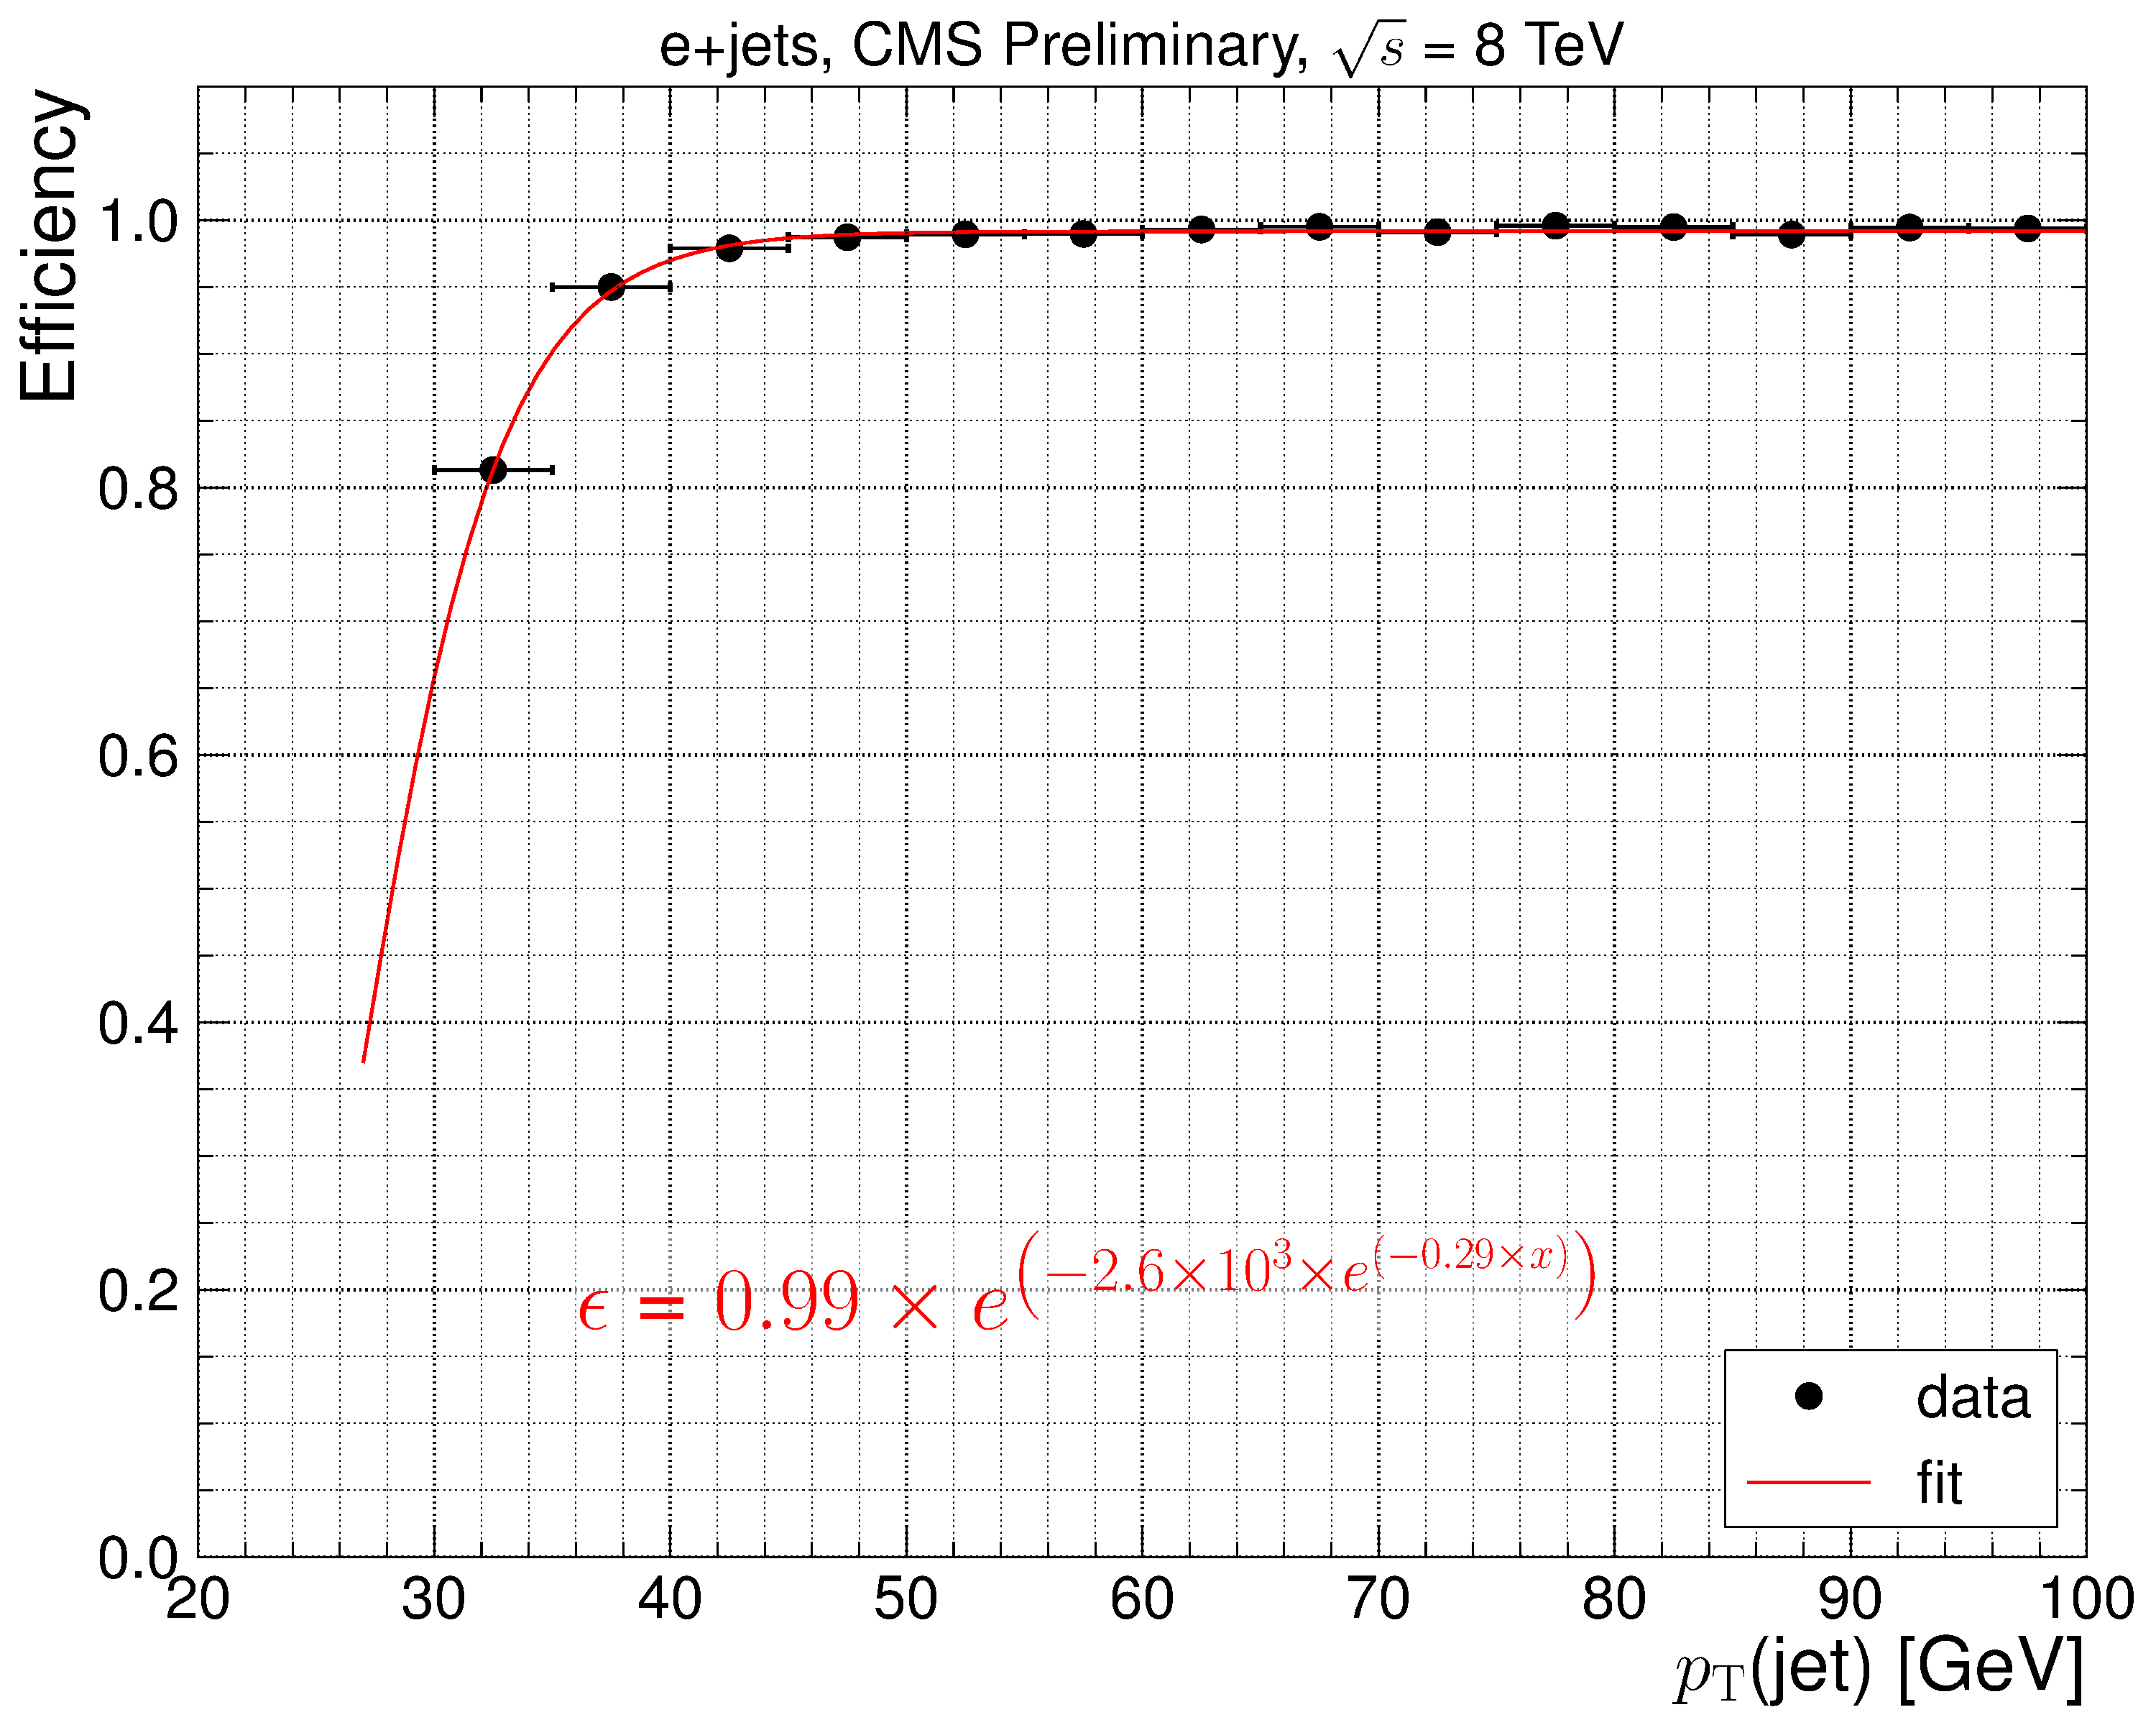
\includegraphics[width=0.48\textwidth]{trigger_eff_pt_uncorr_30.pdf}}
  \hfill
  \subfloat[]{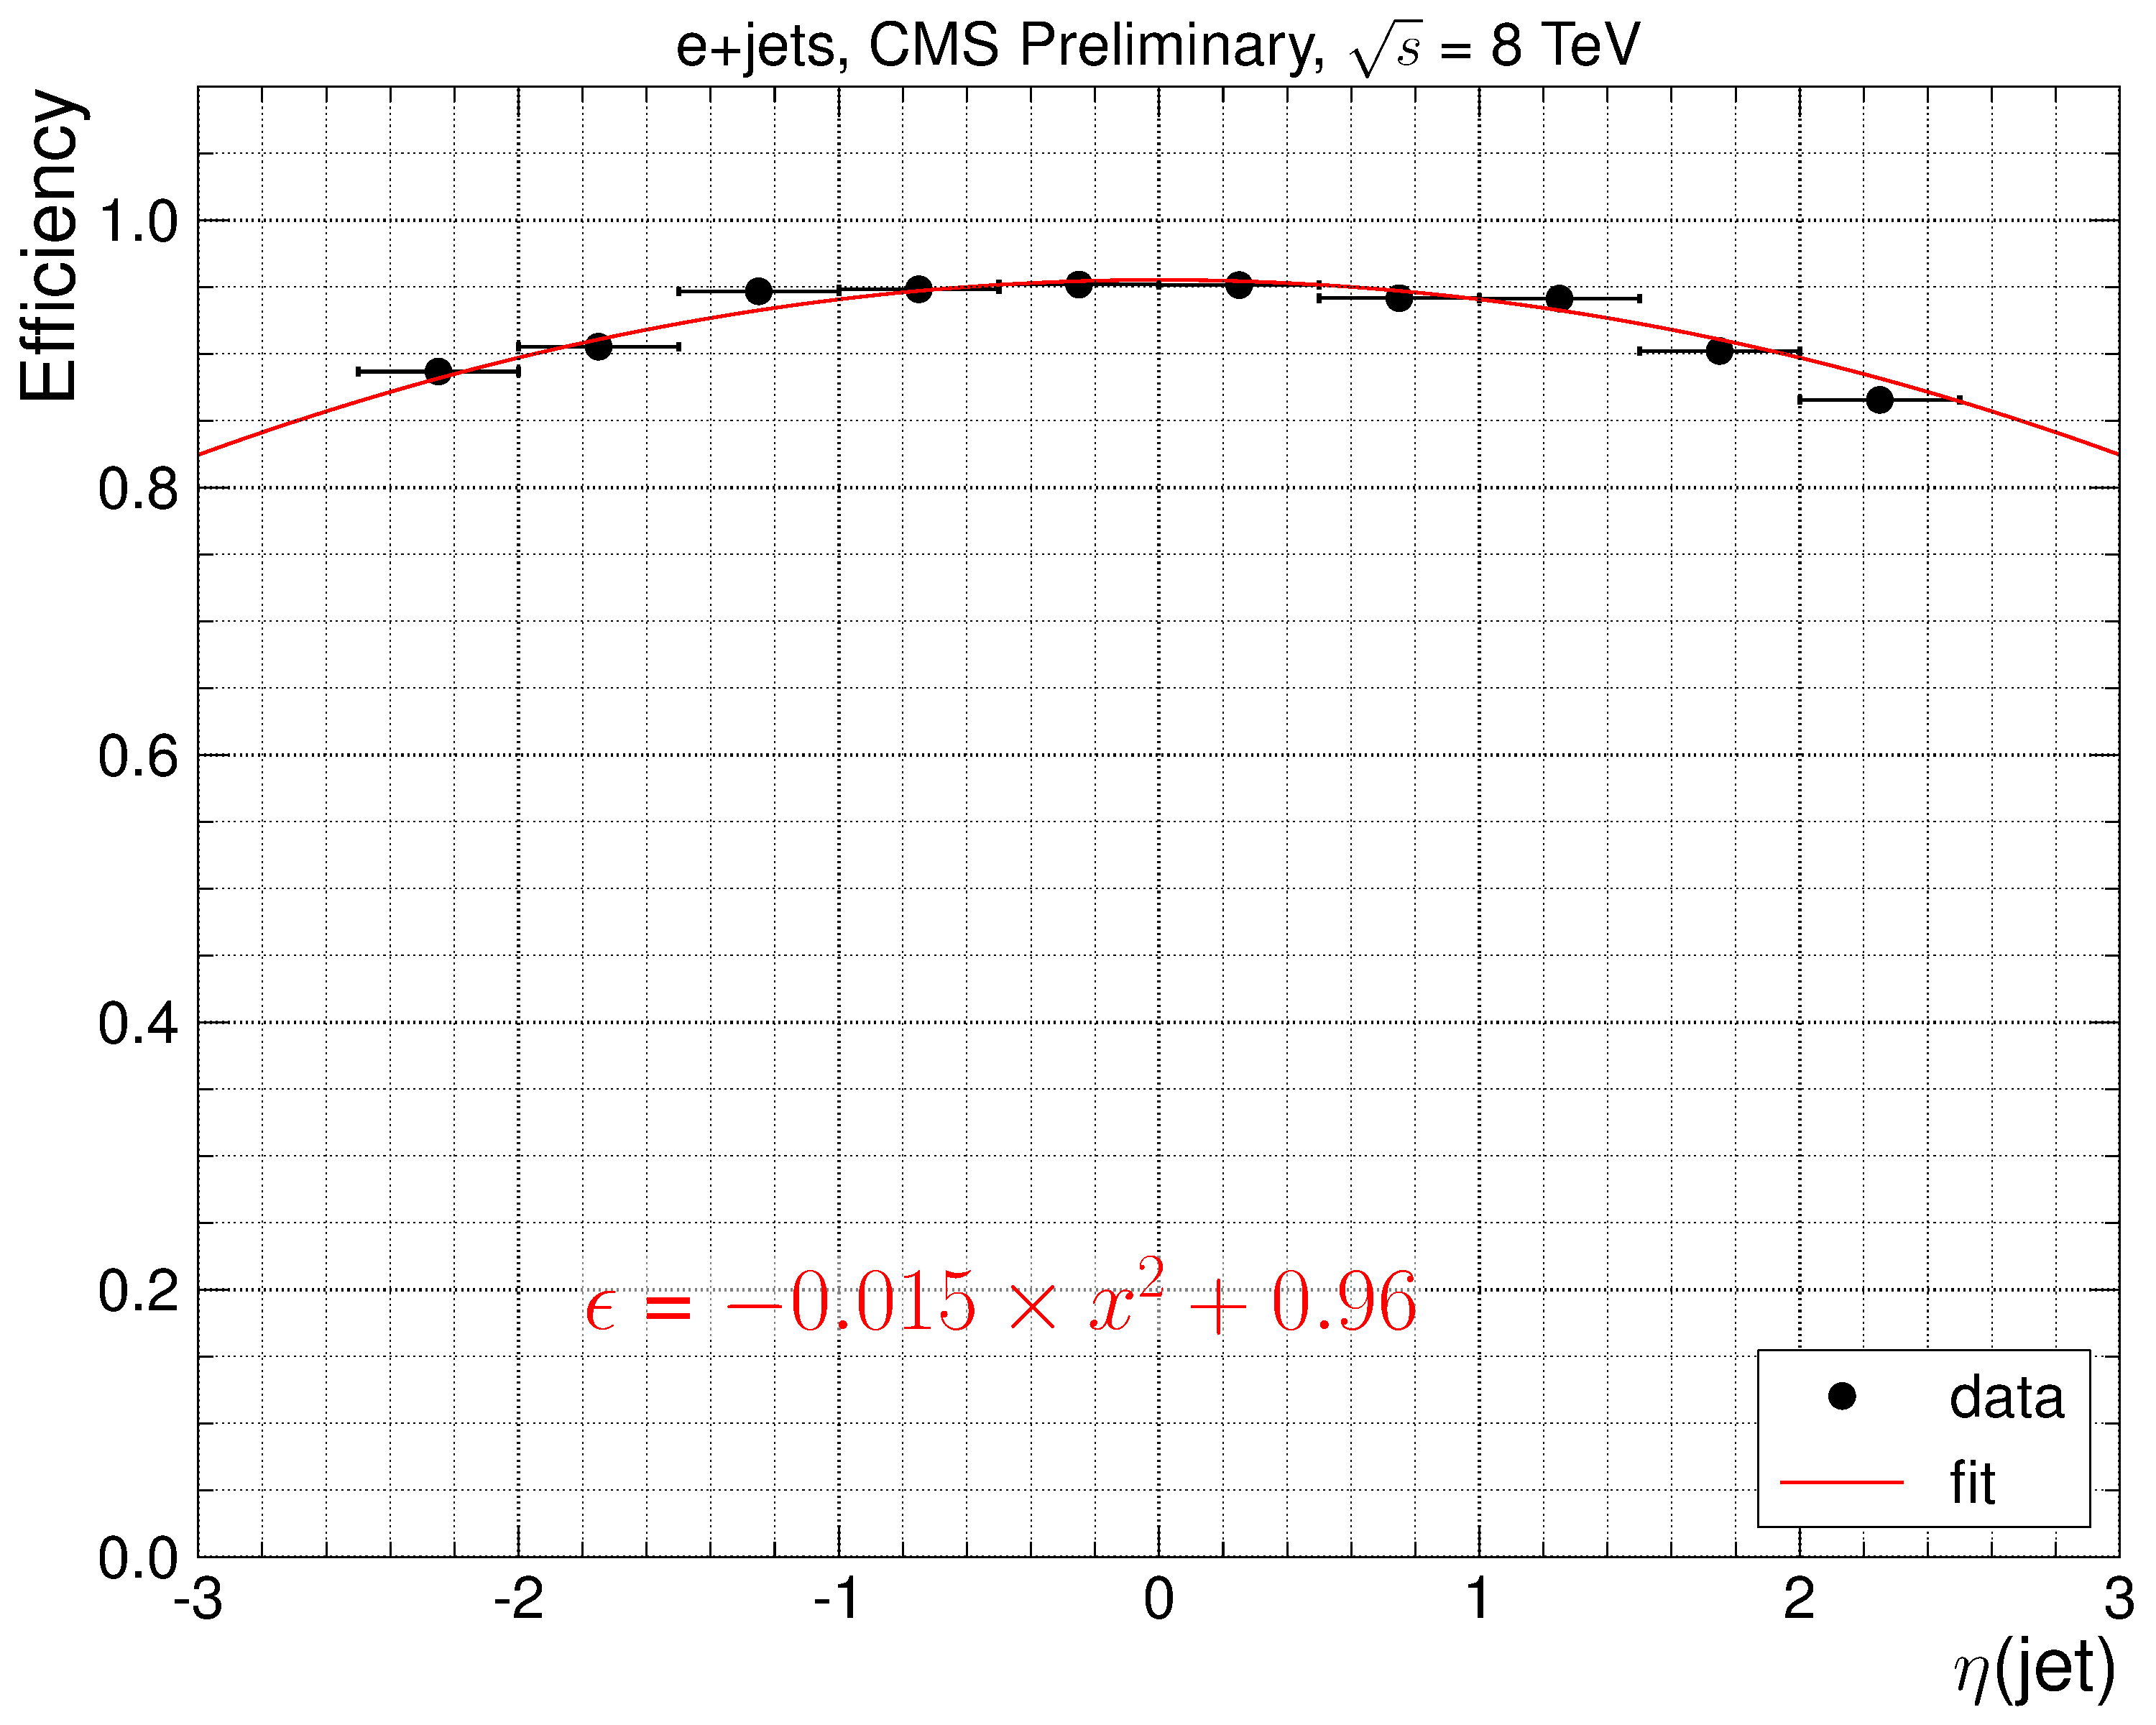
\includegraphics[width=0.48\textwidth]{trigger_eff_eta_uncorr_30.pdf}}
  \caption[Trigger efficiency for \HLTThreeCentralPFJet as a function of the third jet \pt and $\eta$]{Trigger
  efficiency for \HLTThreeCentralPFJet (uncorrected) as a function of the third jet \pt (a) and $\eta$ (b) for events
  with at least three jets.}
\label{fig:top_hlt_pt_eta_3jets} 
\end{figure}

It has to be emphasised that only efficiencies with respect to offline selection with at least three jets were affected.
Requiring a fourth jet in the event increases the trigger efficiency to nearly \SI{100}{\percent}, as can be seen on
Figure~\ref{fig:top_hlt_pt_eta_4jets}. This implies that observed inefficiency in the endcap region was not critical for
analyses requiring at least four jets in the event (including the ones in this thesis), however, it was still important
to investigate this effect in order to better understand any possible systematic errors due to the triggering.

\begin{figure}[hbtp]
  \centering
  \subfloat[]{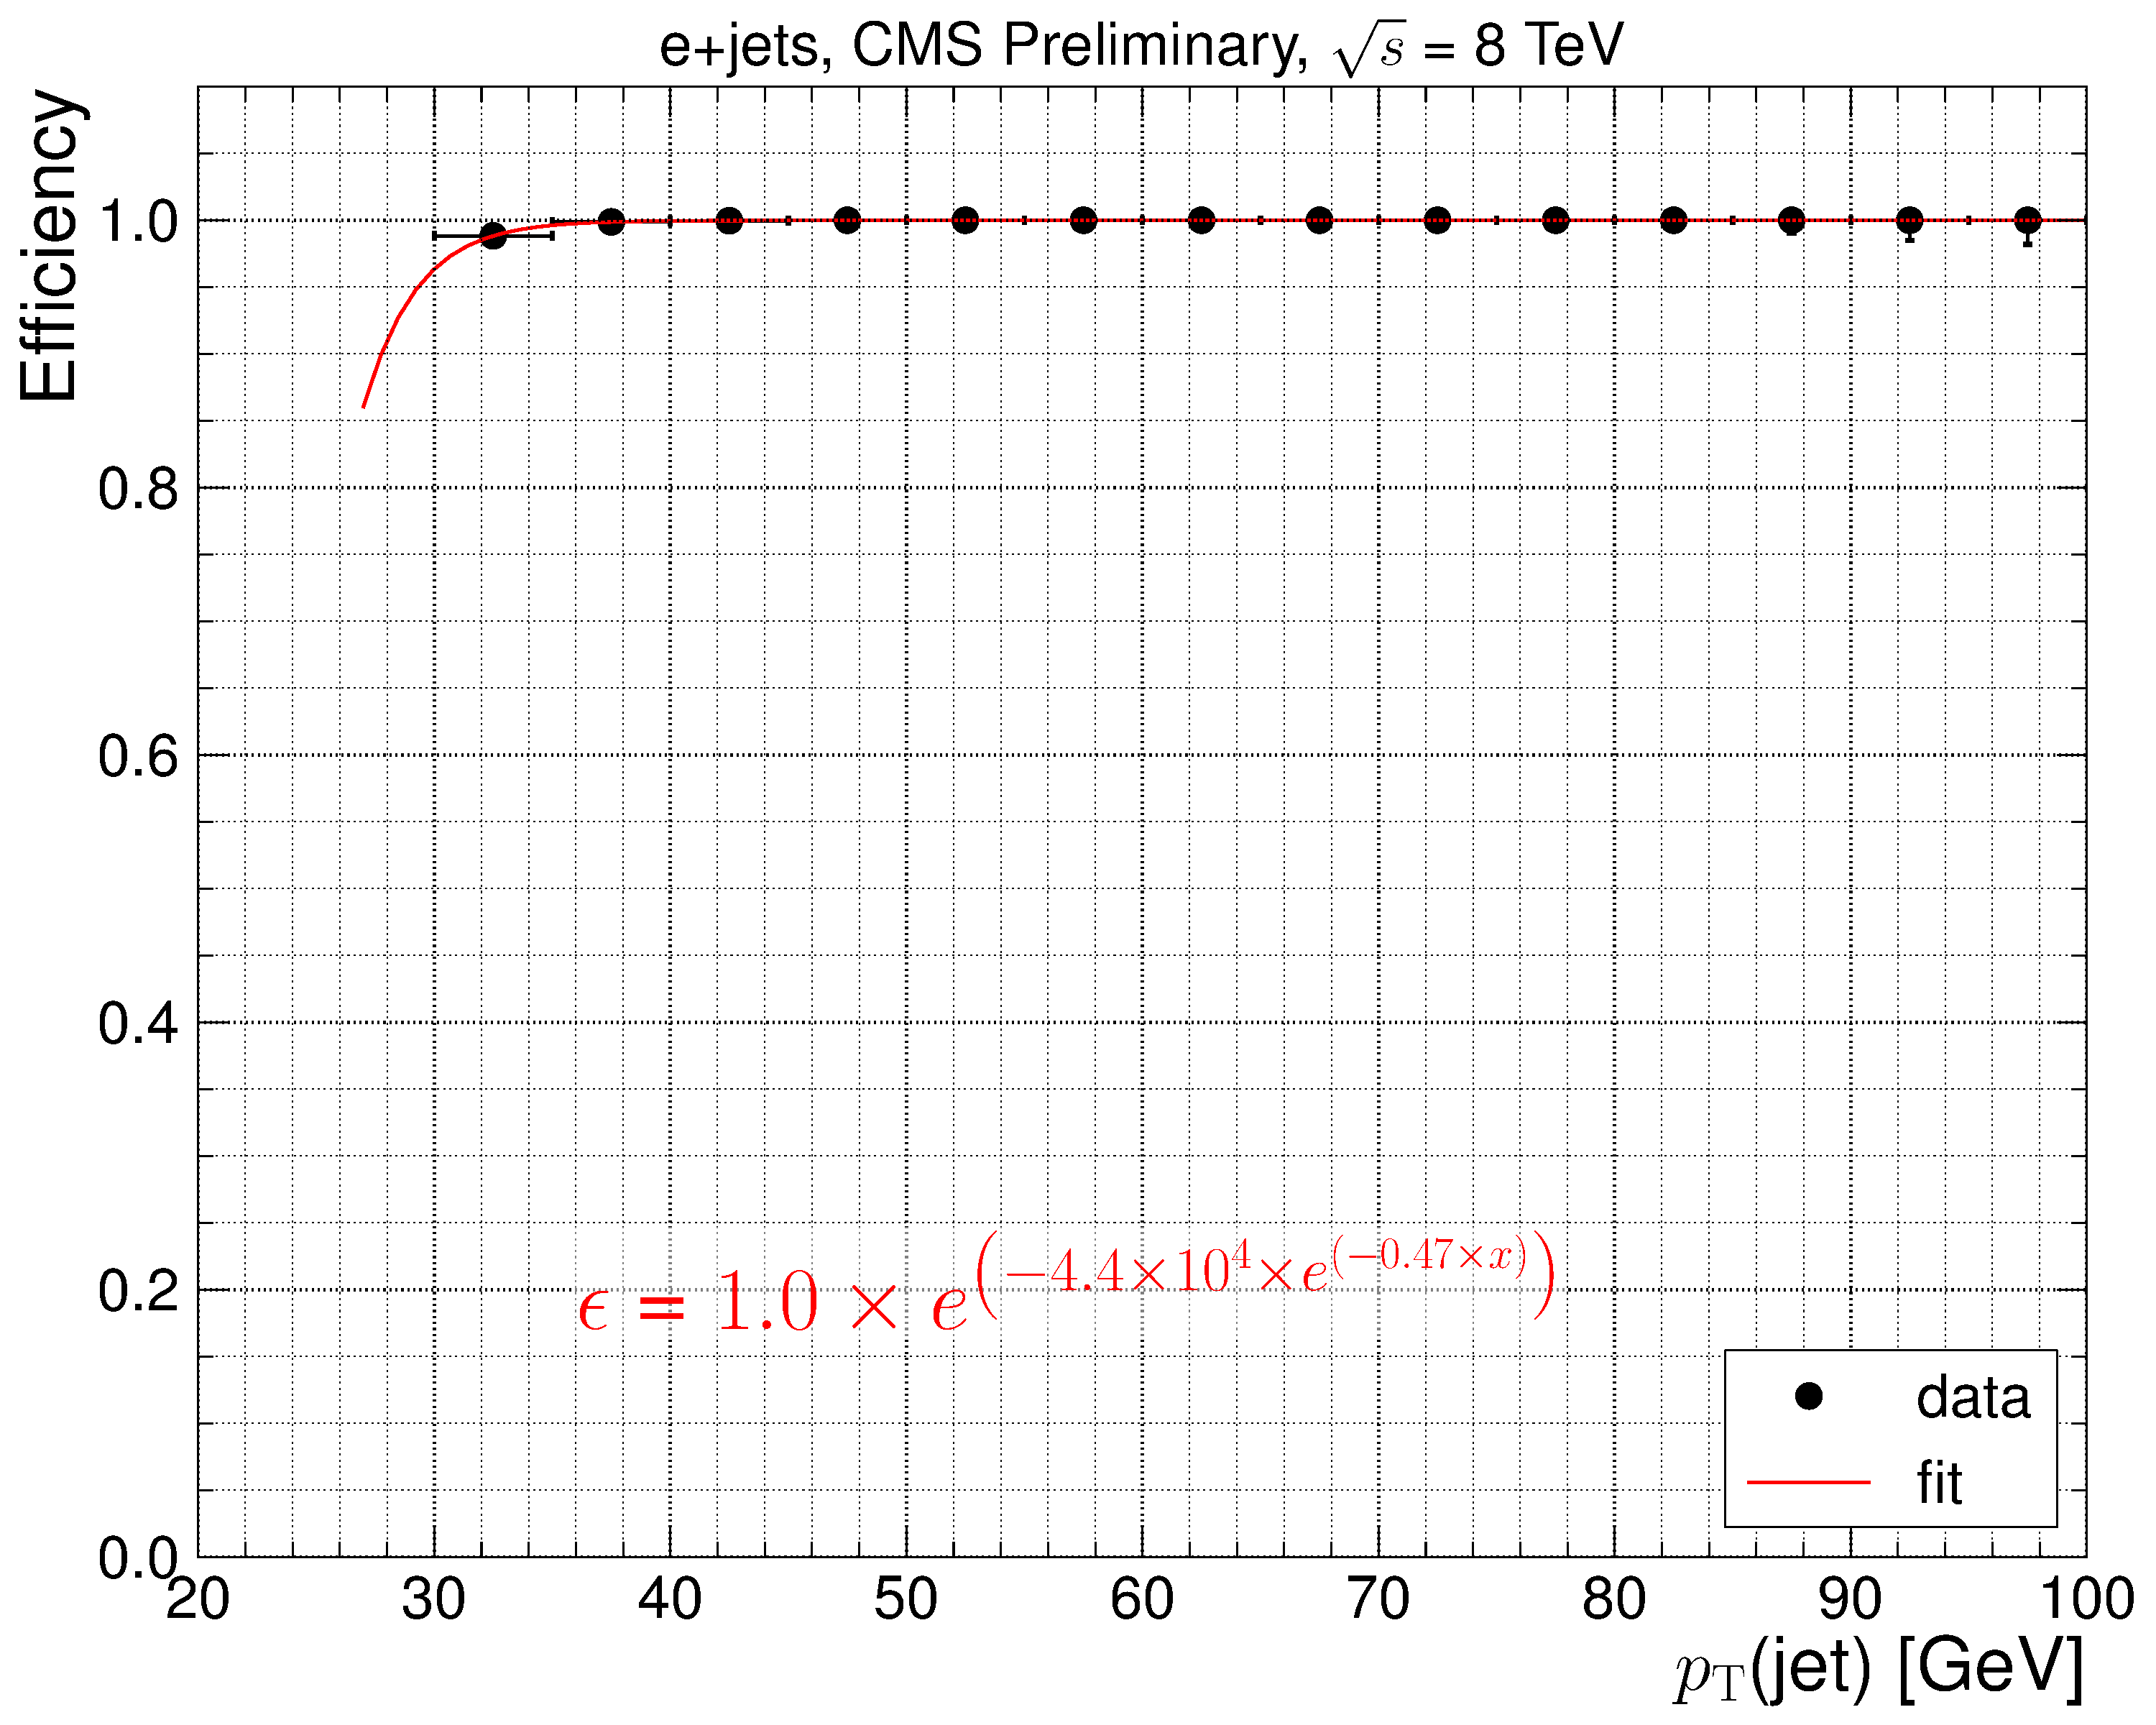
\includegraphics[width=0.48\textwidth]{trigger_eff_pt_uncorr_4th_30.pdf}}
  \hfill
  \subfloat[]{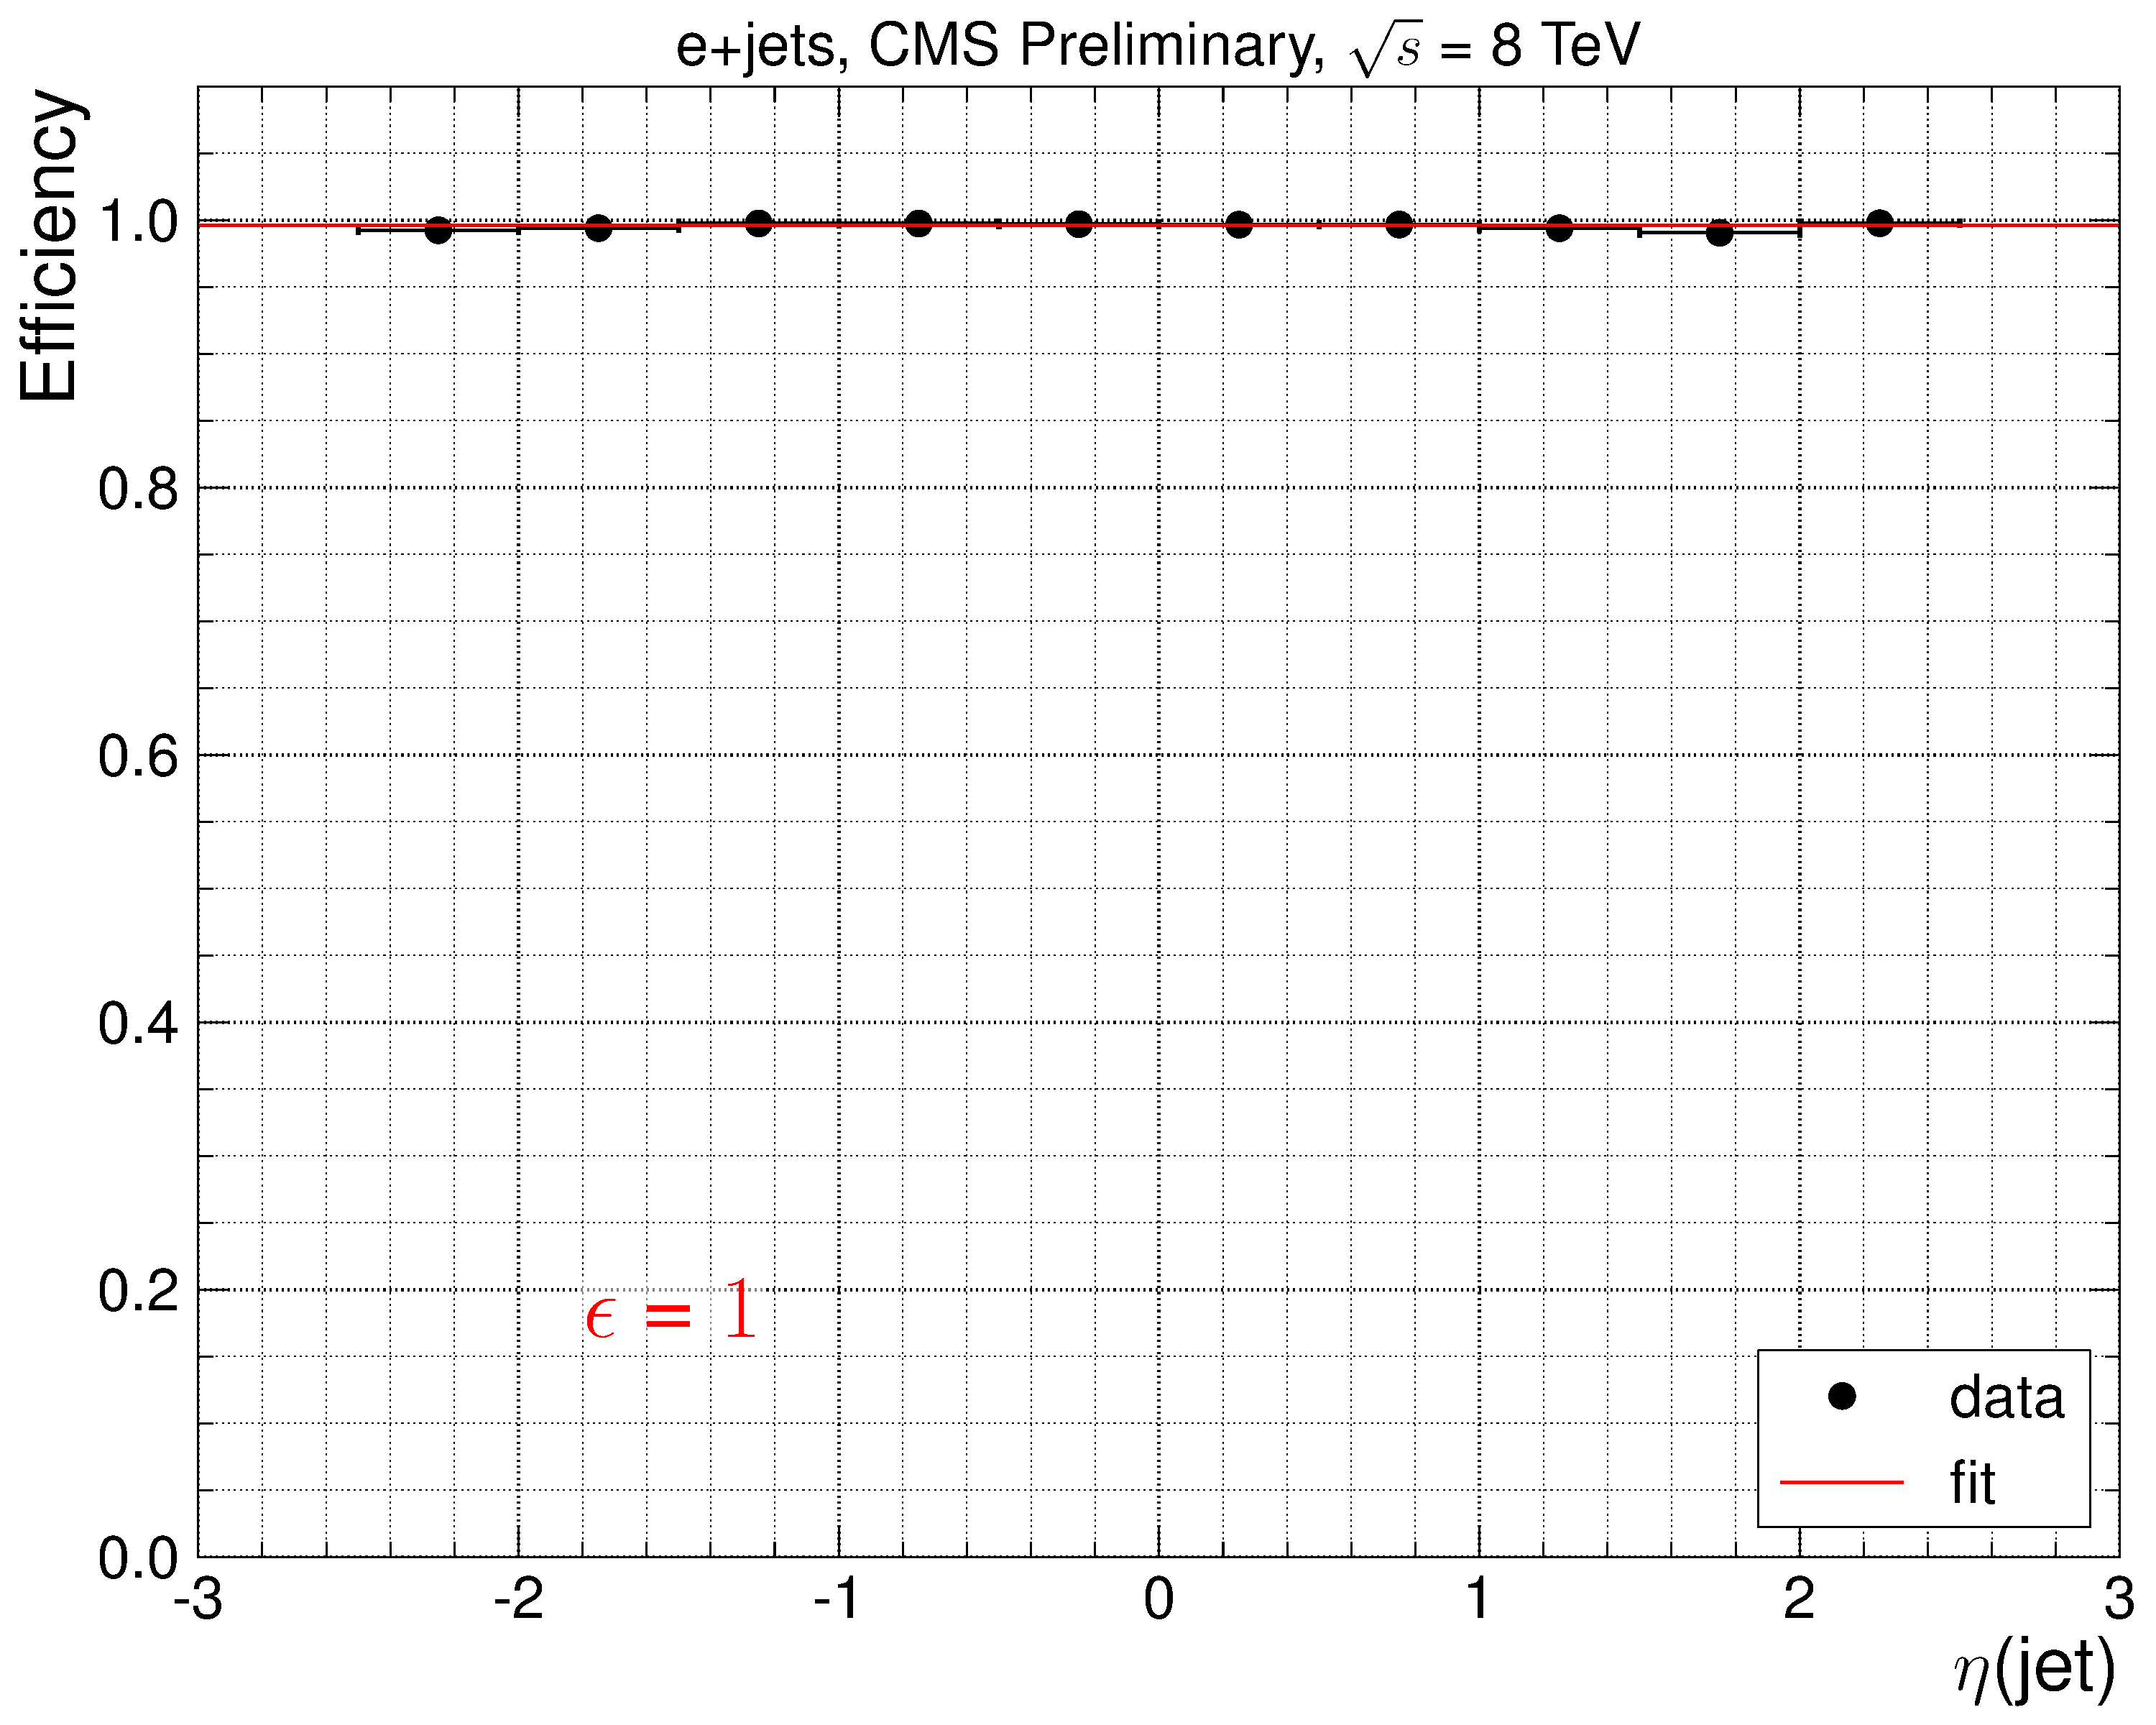
\includegraphics[width=0.48\textwidth]{trigger_eff_eta_uncorr_4th_30.pdf}}
  \caption[Trigger efficiency for \HLTThreeCentralPFJet as a function of the third jet \pt and $\eta$]{Trigger
  efficiency for \HLTThreeCentralPFJet (uncorrected) as a function of the third jet \pt (a) and $\eta$ (b) for events
  with at least four jets.}
\label{fig:top_hlt_pt_eta_4jets} 
\end{figure}


For the purpose of the study, a modified HLT menu was created, containing new versions of the main signal trigger with
jet energy corrections and charged hadron subtraction applied. This menu was run on a \ttbar skim of a RAW dataset
mentioned above, and the resulting trigger flags as well as jet collections were used to produce the final plots.

Figure~\ref{fig:top_hlt_pt_eta_JEC_3jets} presents the results for the aforementioned trigger path but with jet energy
corrections applied, and Figure~\ref{fig:top_hlt_pt_eta_JEC_PFnoPU_3jets} shows it for the same path with both charged
hadron subtraction and jet corrections applied. It is obvious that all these corrections haven't solved the inefficiency
problem in the endcaps, which caused some confusion in the group that provided them and triggered additional scrutiny
from the trigger and jet/\MET experts.

\begin{figure}[hbtp]
  \centering
  \subfloat[]{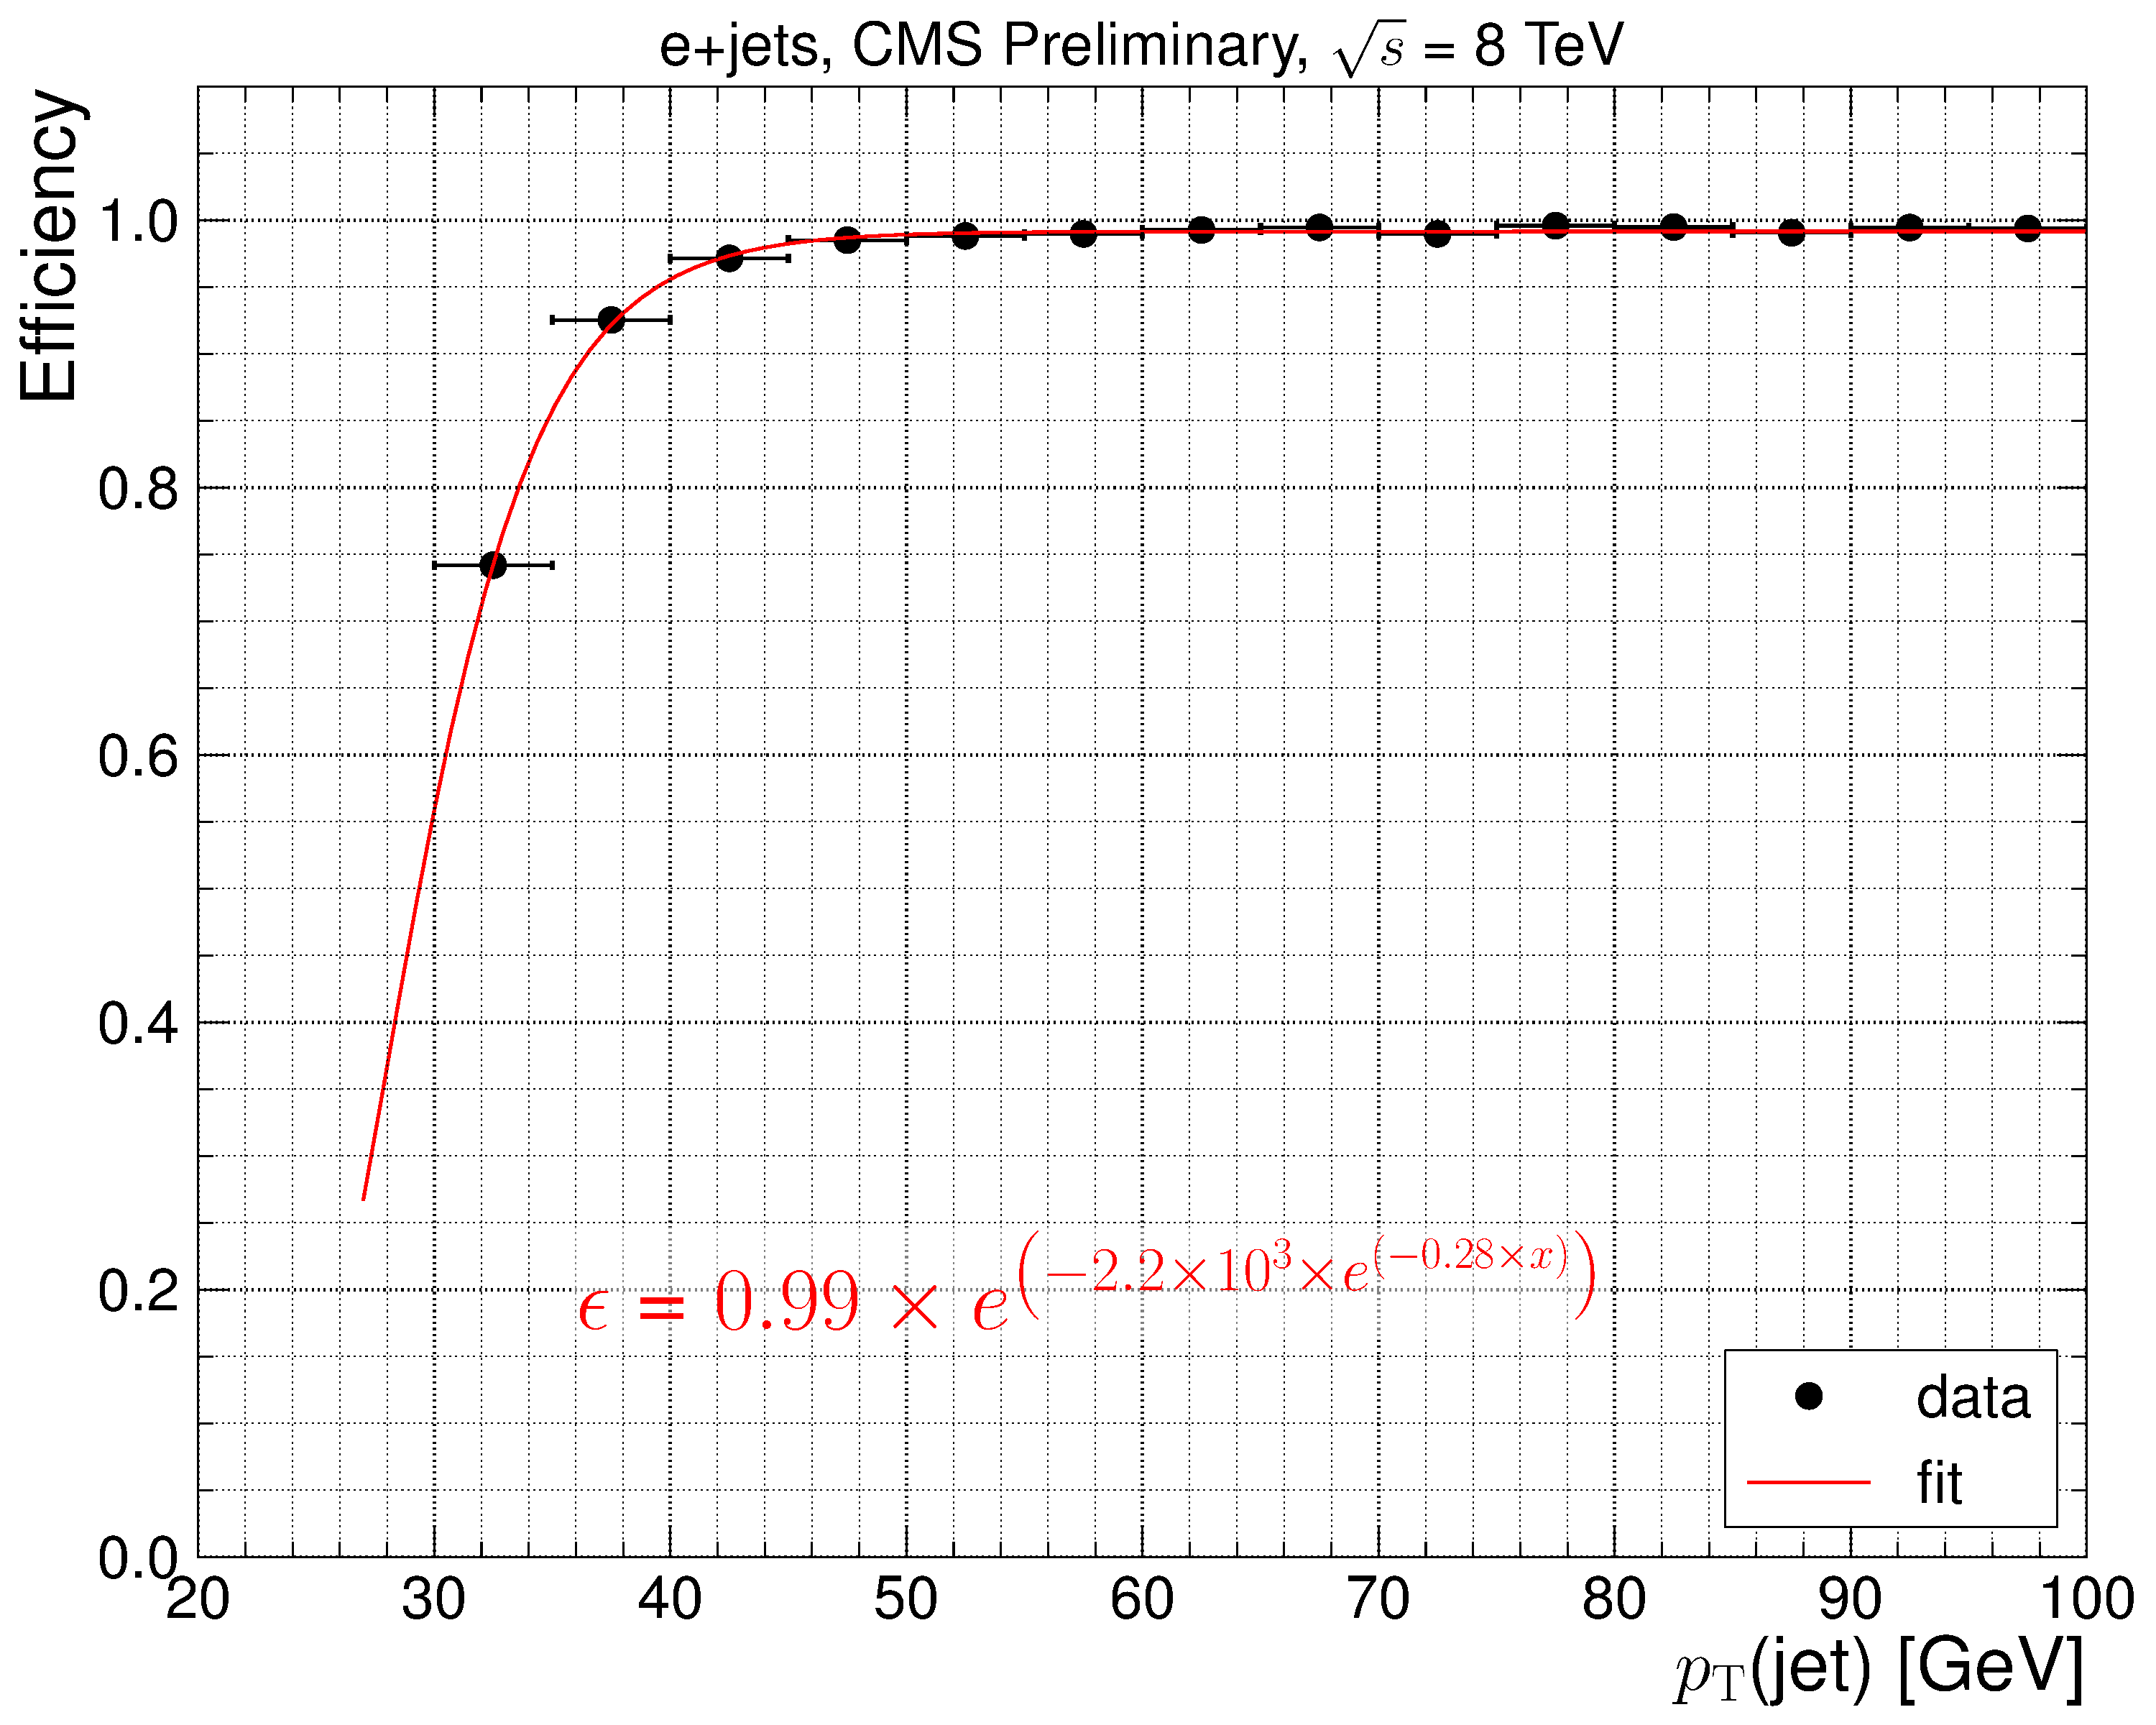
\includegraphics[width=0.48\textwidth]{trigger_eff_pt_JEC_30.pdf}}
  \hfill
  \subfloat[]{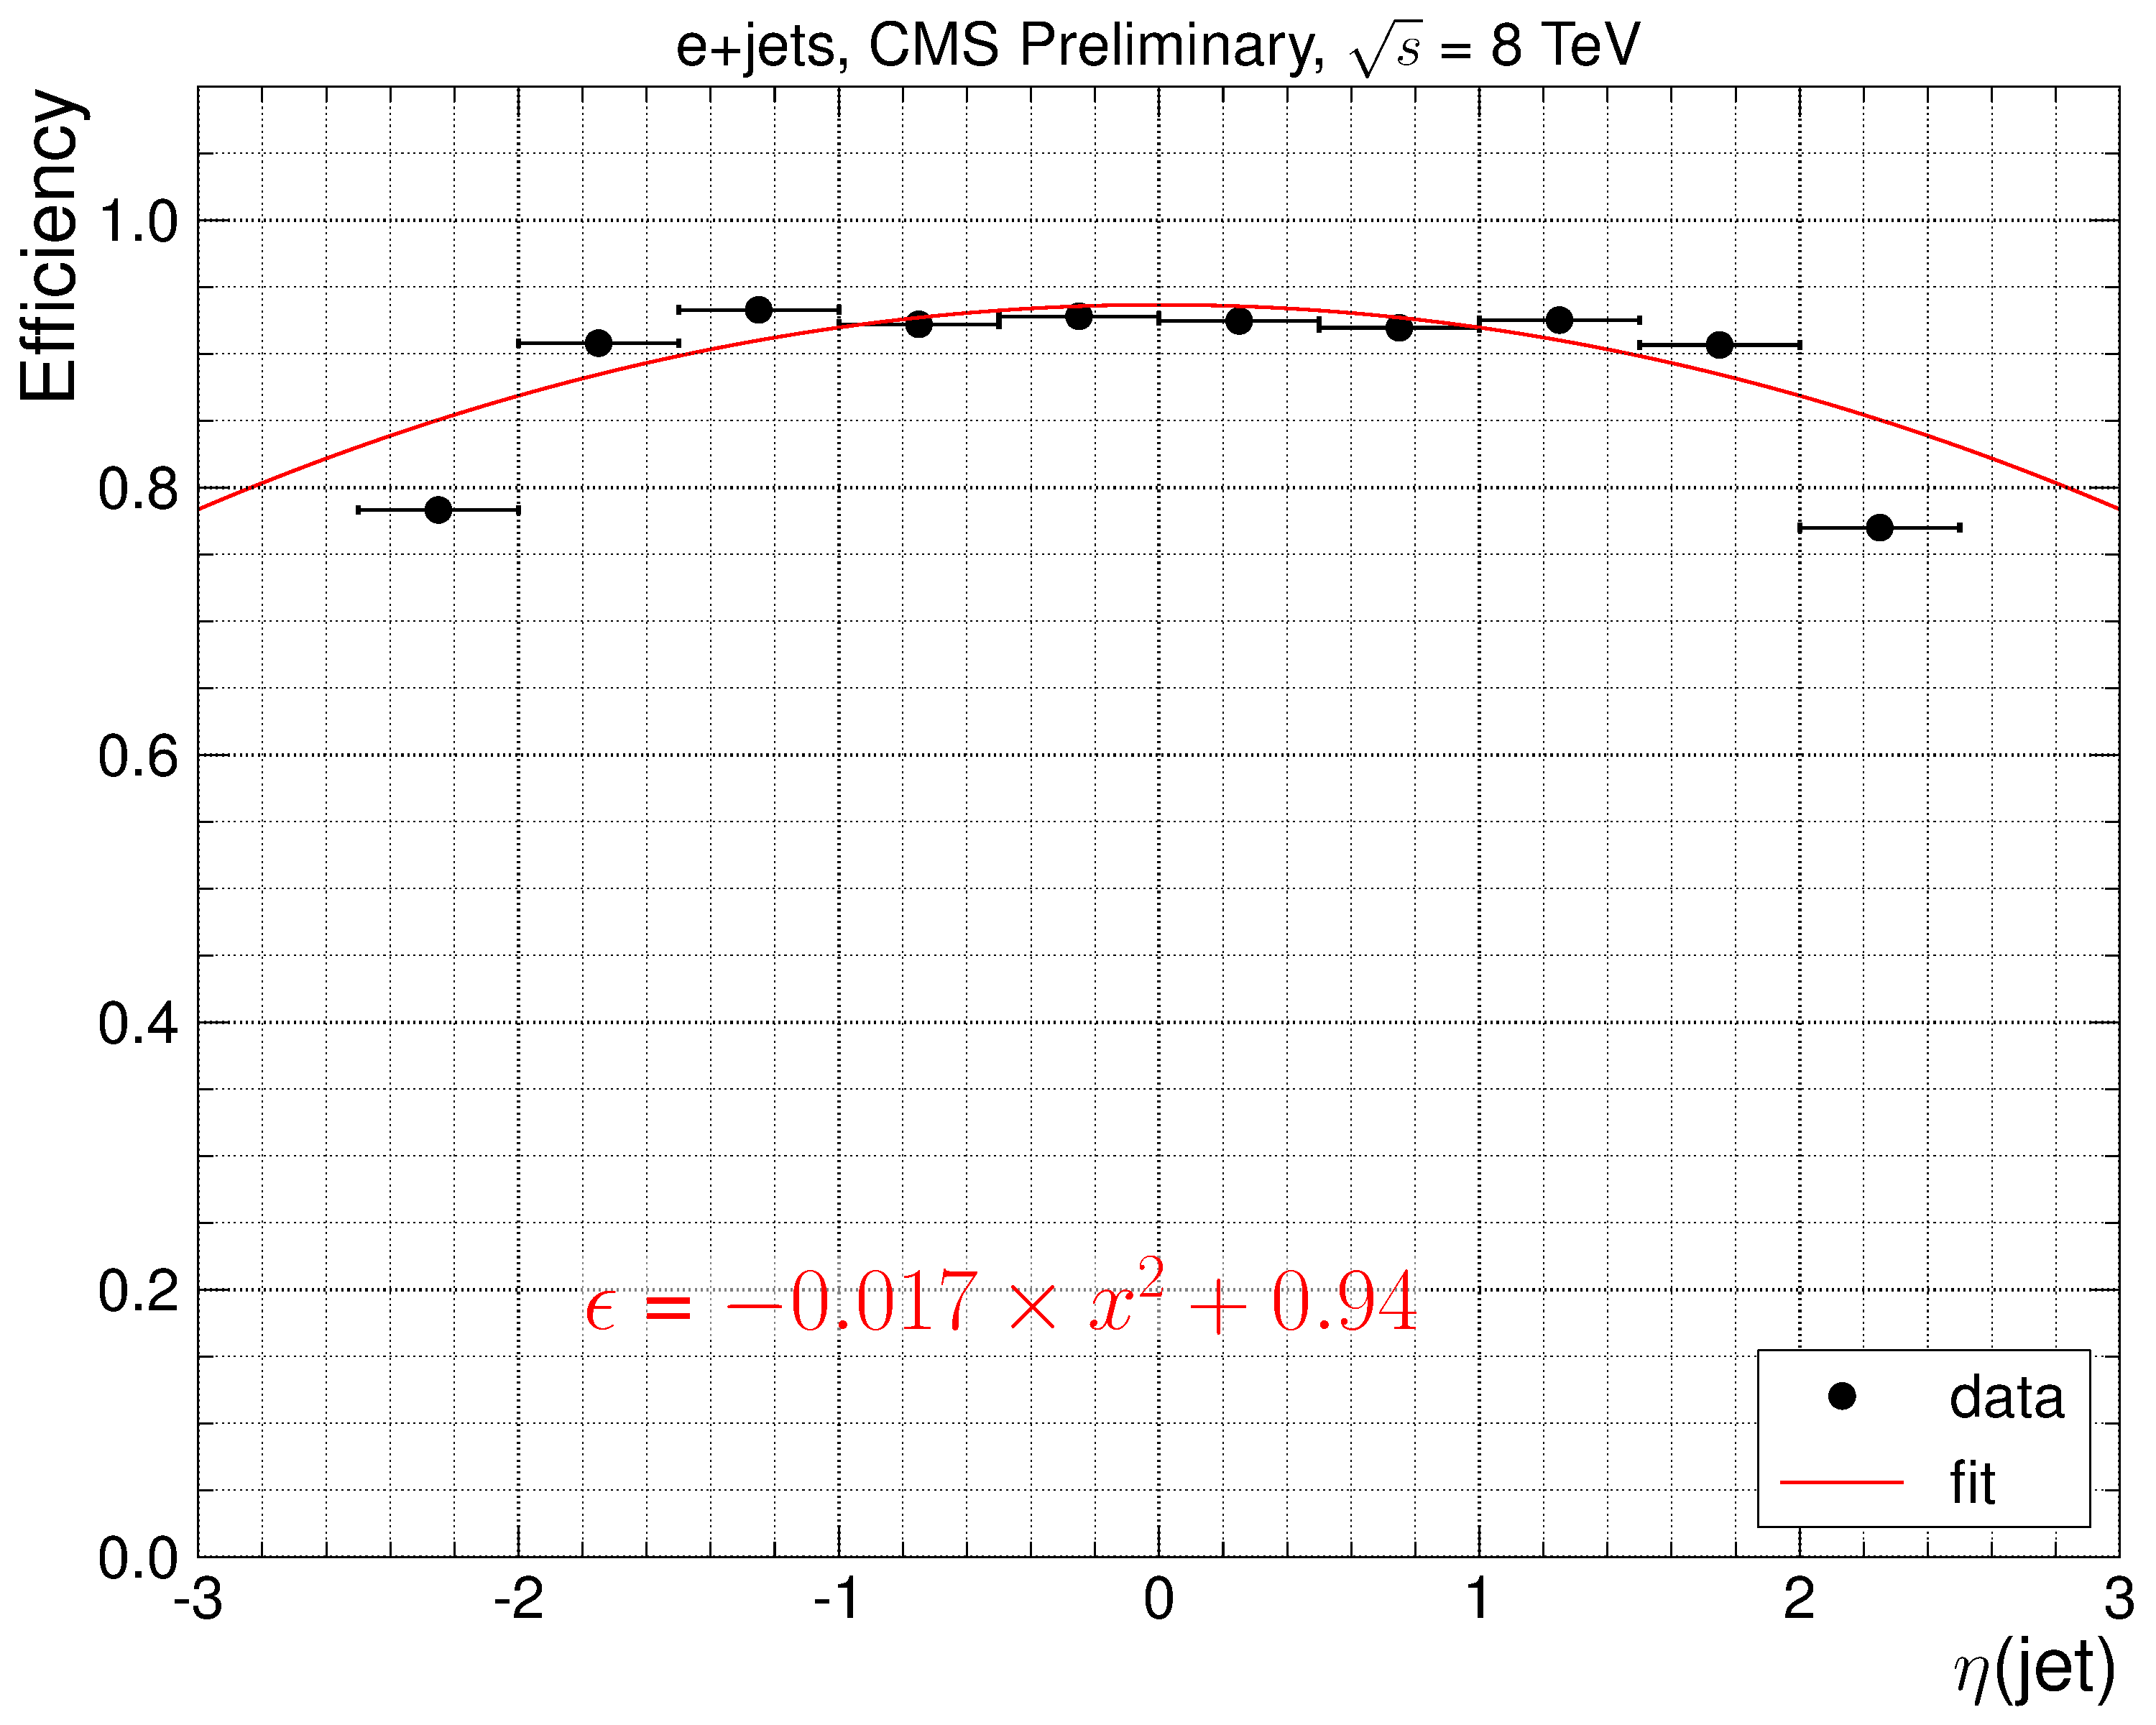
\includegraphics[width=0.48\textwidth]{trigger_eff_eta_JEC_30.pdf}}
  \caption[Trigger efficiency for \HLTThreeCentralPFJet as a function of the third jet \pt and $\eta$]{Trigger
  efficiency for \HLTThreeCentralPFJet with jet energy corrections applied online, as a function of the third jet \pt (a) and $\eta$
  (b) for events with at least three jets.}
\label{fig:top_hlt_pt_eta_JEC_3jets} 
\end{figure}

\begin{figure}[hbtp]
  \centering
  \subfloat[]{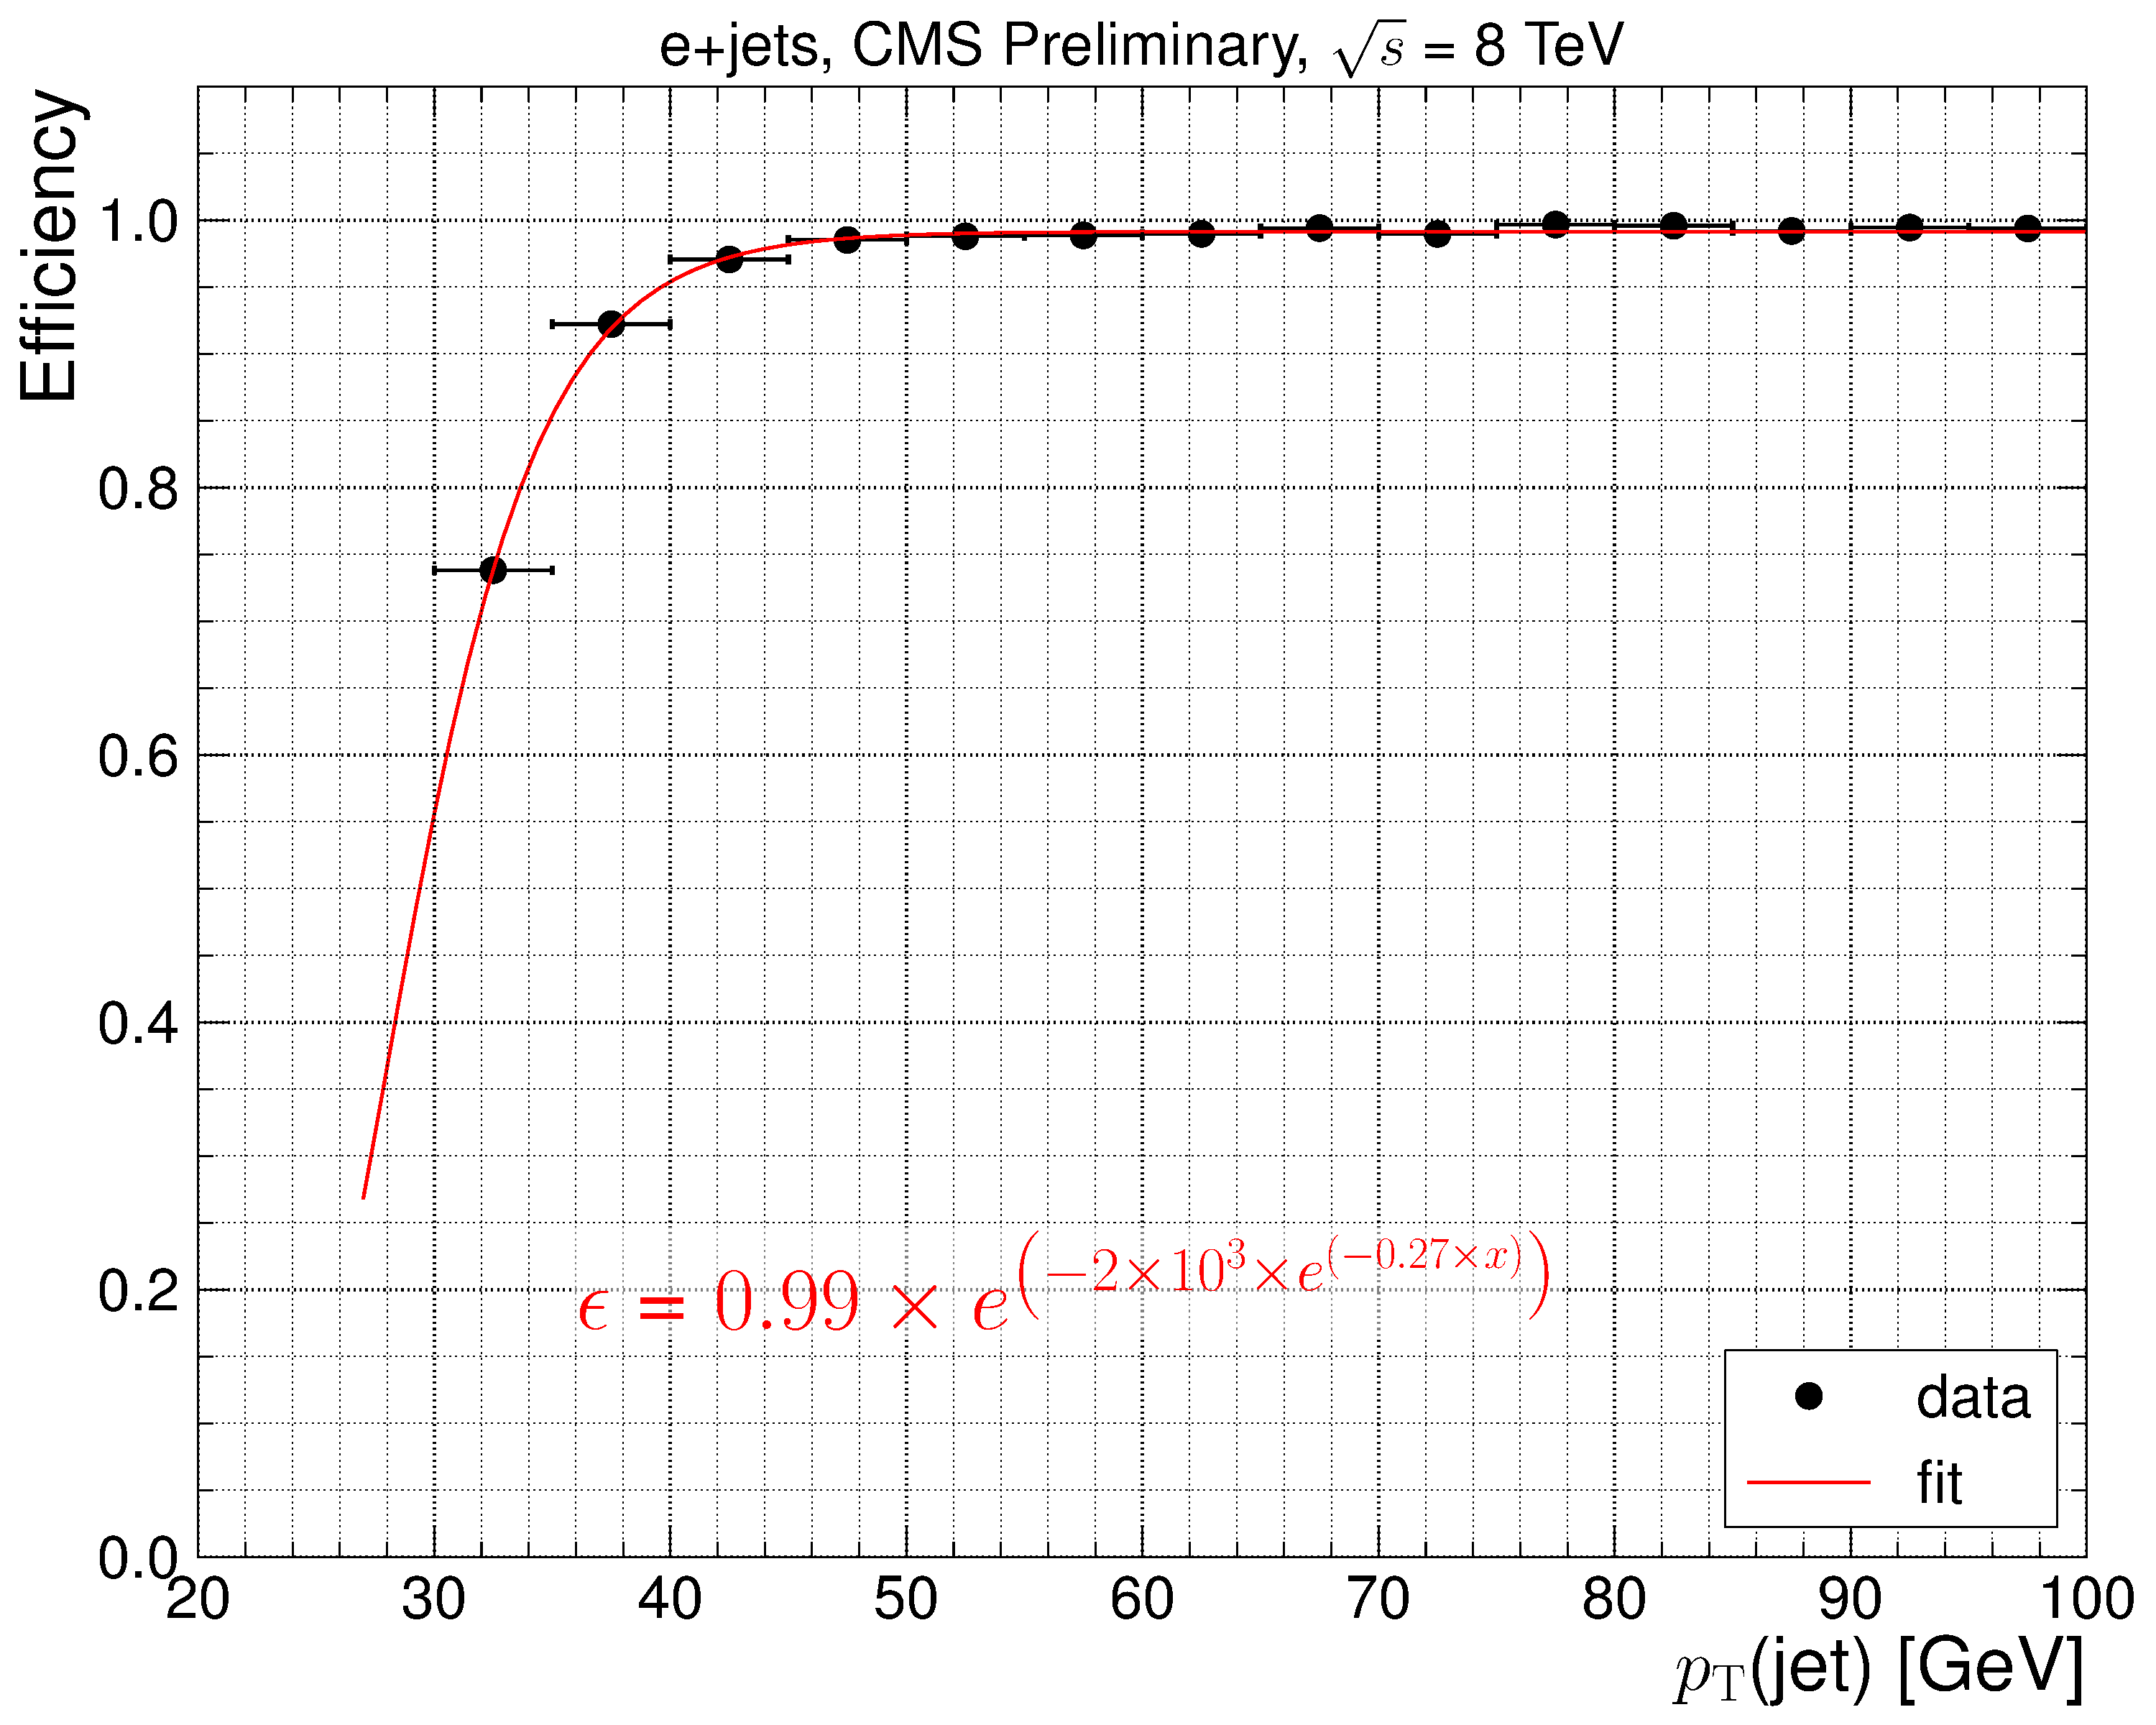
\includegraphics[width=0.48\textwidth]{trigger_eff_pt_JEC_PFnoPU_30.pdf}}
  \hfill
  \subfloat[]{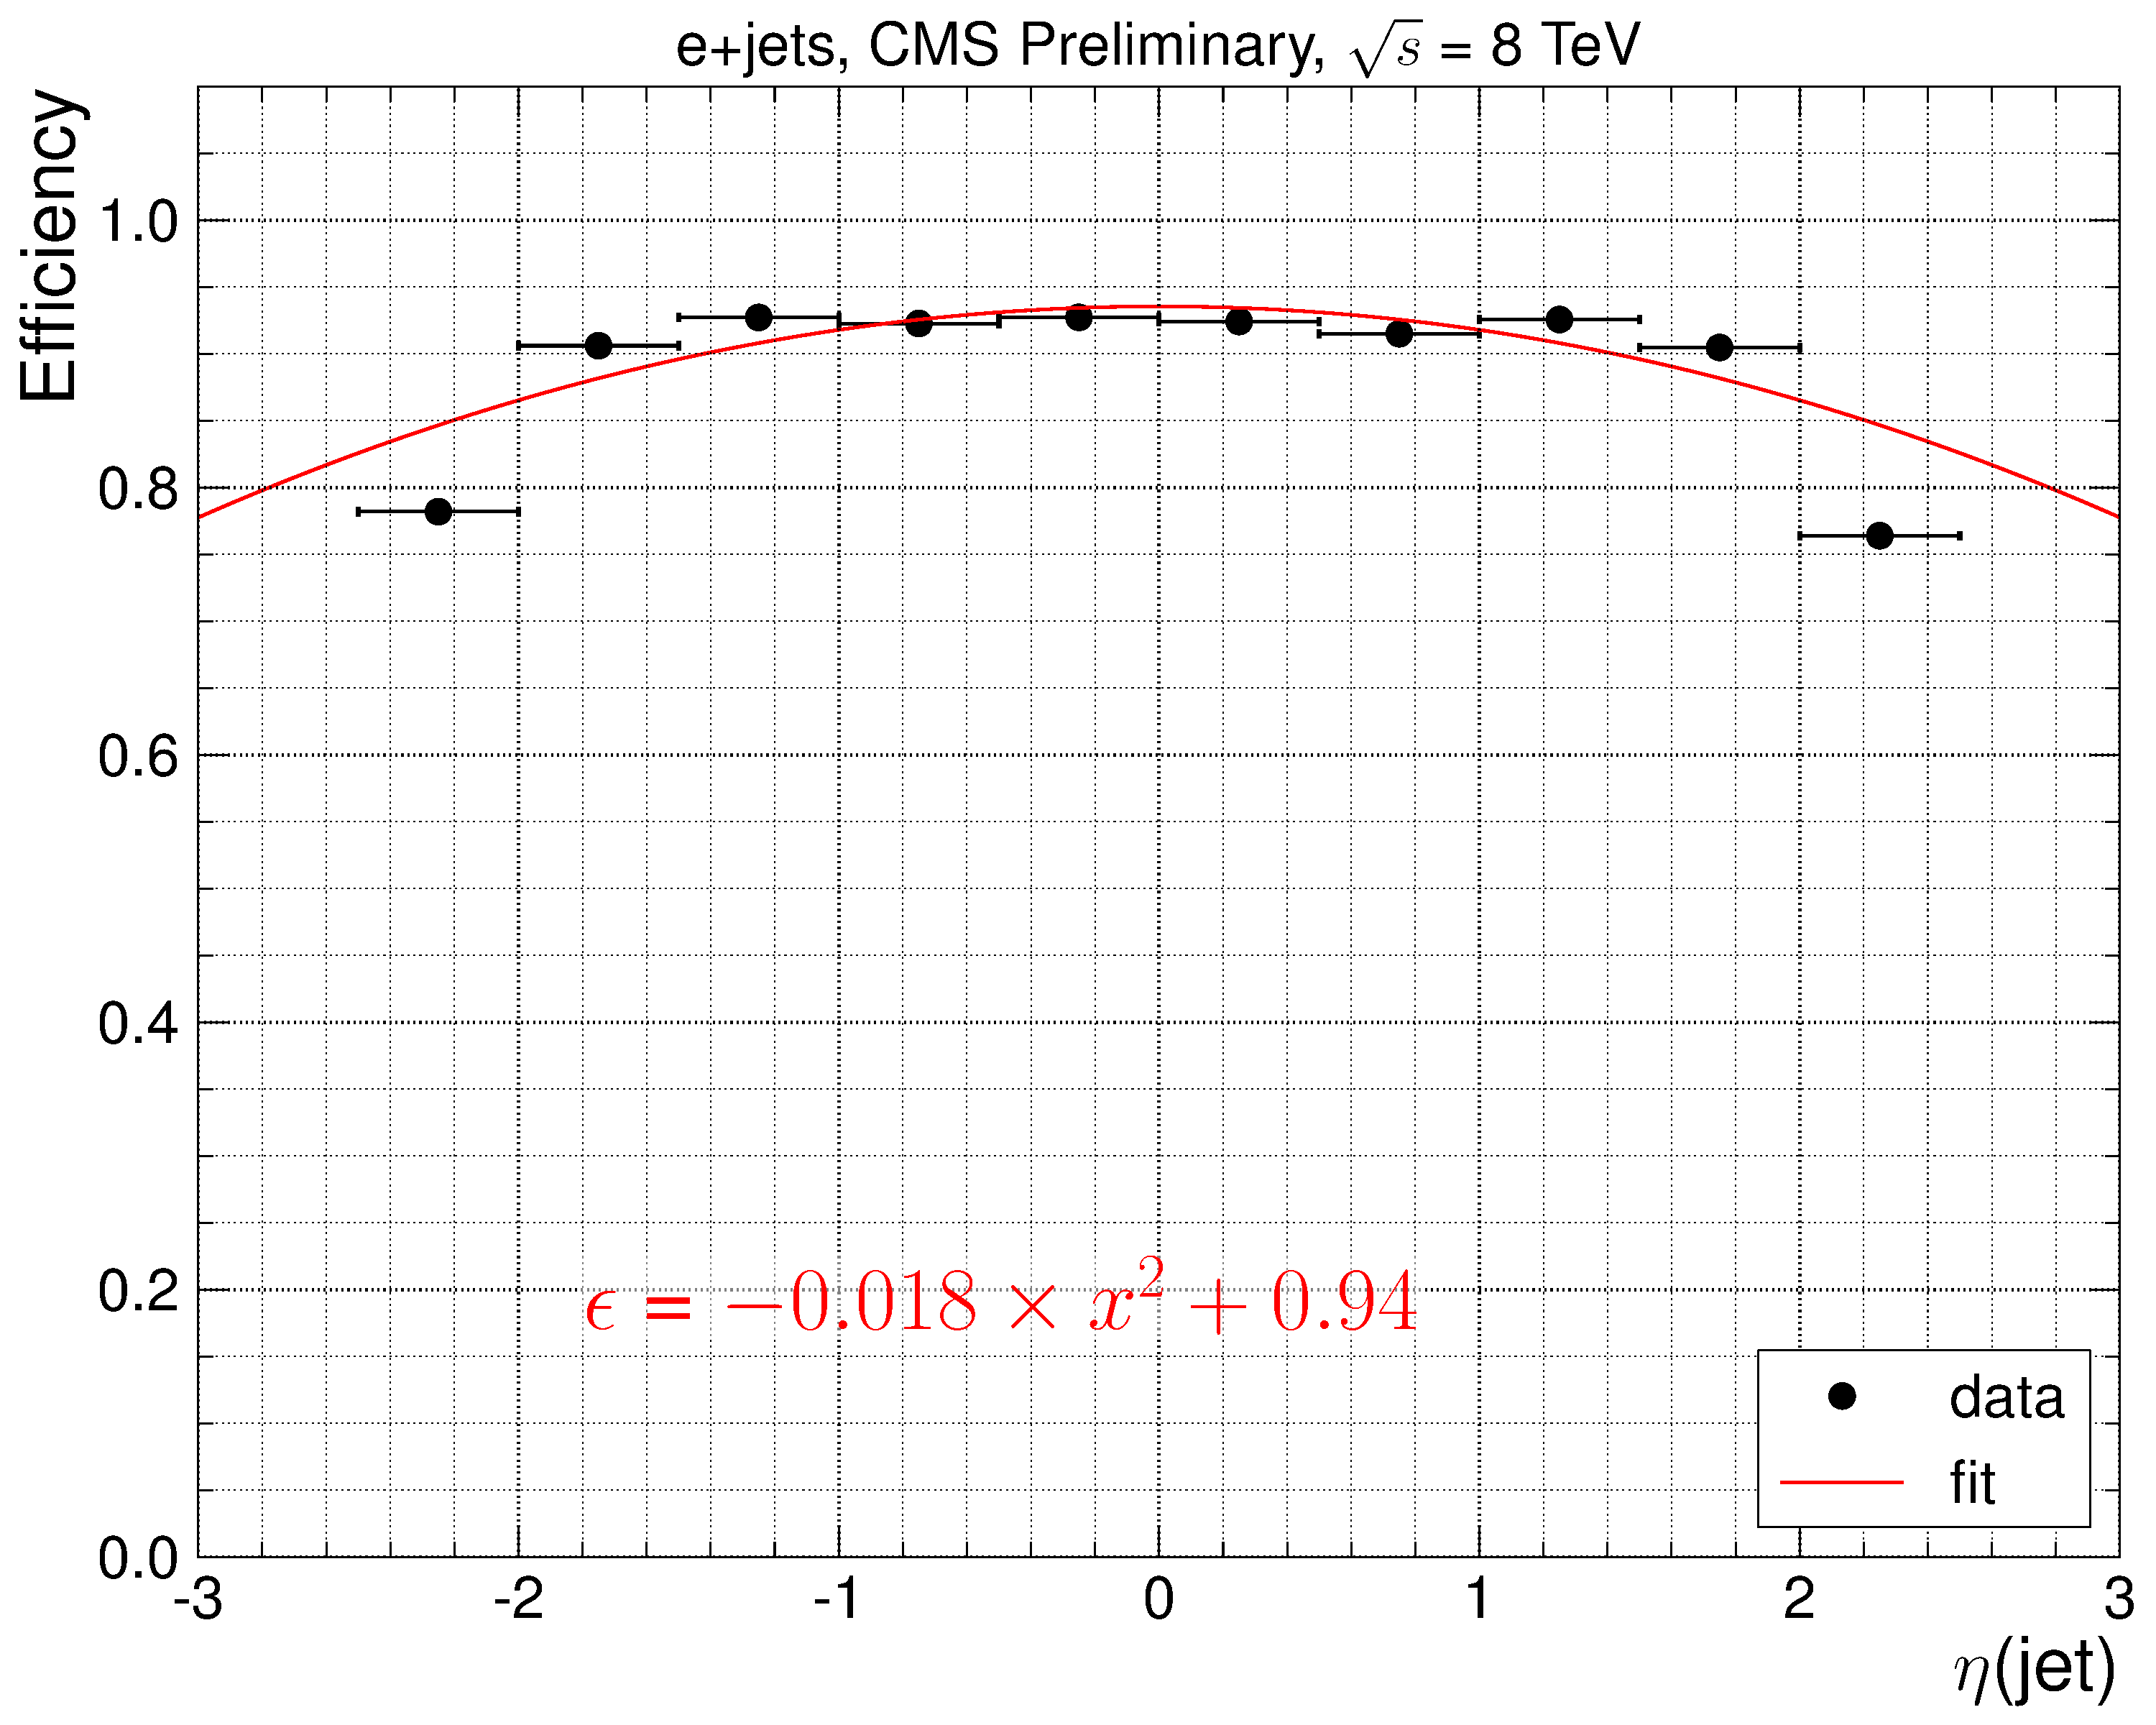
\includegraphics[width=0.48\textwidth]{trigger_eff_eta_JEC_PFnoPU_30.pdf}}
  \caption[Trigger efficiency for \HLTThreeCentralPFJet as a function of the third jet \pt and $\eta$]{Trigger efficiency for
  \HLTThreeCentralPFJet with jet energy corrections and charged hadron subtraction applied online, as a function of the
  third jet \pt (a) and $\eta$ (b) for events with at least three jets.}
\label{fig:top_hlt_pt_eta_JEC_PFnoPU_3jets} 
\end{figure}

In order to gain further understanding, jet response distributions were investigated. Jet response is a ratio of the
transverse momenta of offline-reconstructed and HLT jets, ideally produced from the same objects in the detector. To
find this ratio, all the HLT jets were matched with offline jets found within a cone of $\Delta R = 0.3$ for each online
jet. Matching efficiency proved to be close to unity, and subsequent distributions were produced only for the
successfully matched jets. Figure~\ref{fig:top_hlt_jet_response} shows the response plots for trigger paths with
different corrections: uncorrected, only jet energy corrected (JEC) and with both jet energy corrections and charged
hadron subtraction (JEC+CHS) applied. It can be seen that corrections work reasonably well in the barrel region, but
substantially underestimate the energy of online jets in the endcap region. The response plot shown in slices of offline
jet transverse momenta (c) suggests that corrections work better for jets with higher energy, which can also be seen
from the distribution with respect to jet \pt, however, the overall response in the endcap region is still far from
being perfect.

 \begin{figure}[hbtp]
  \centering
  \subfloat[]{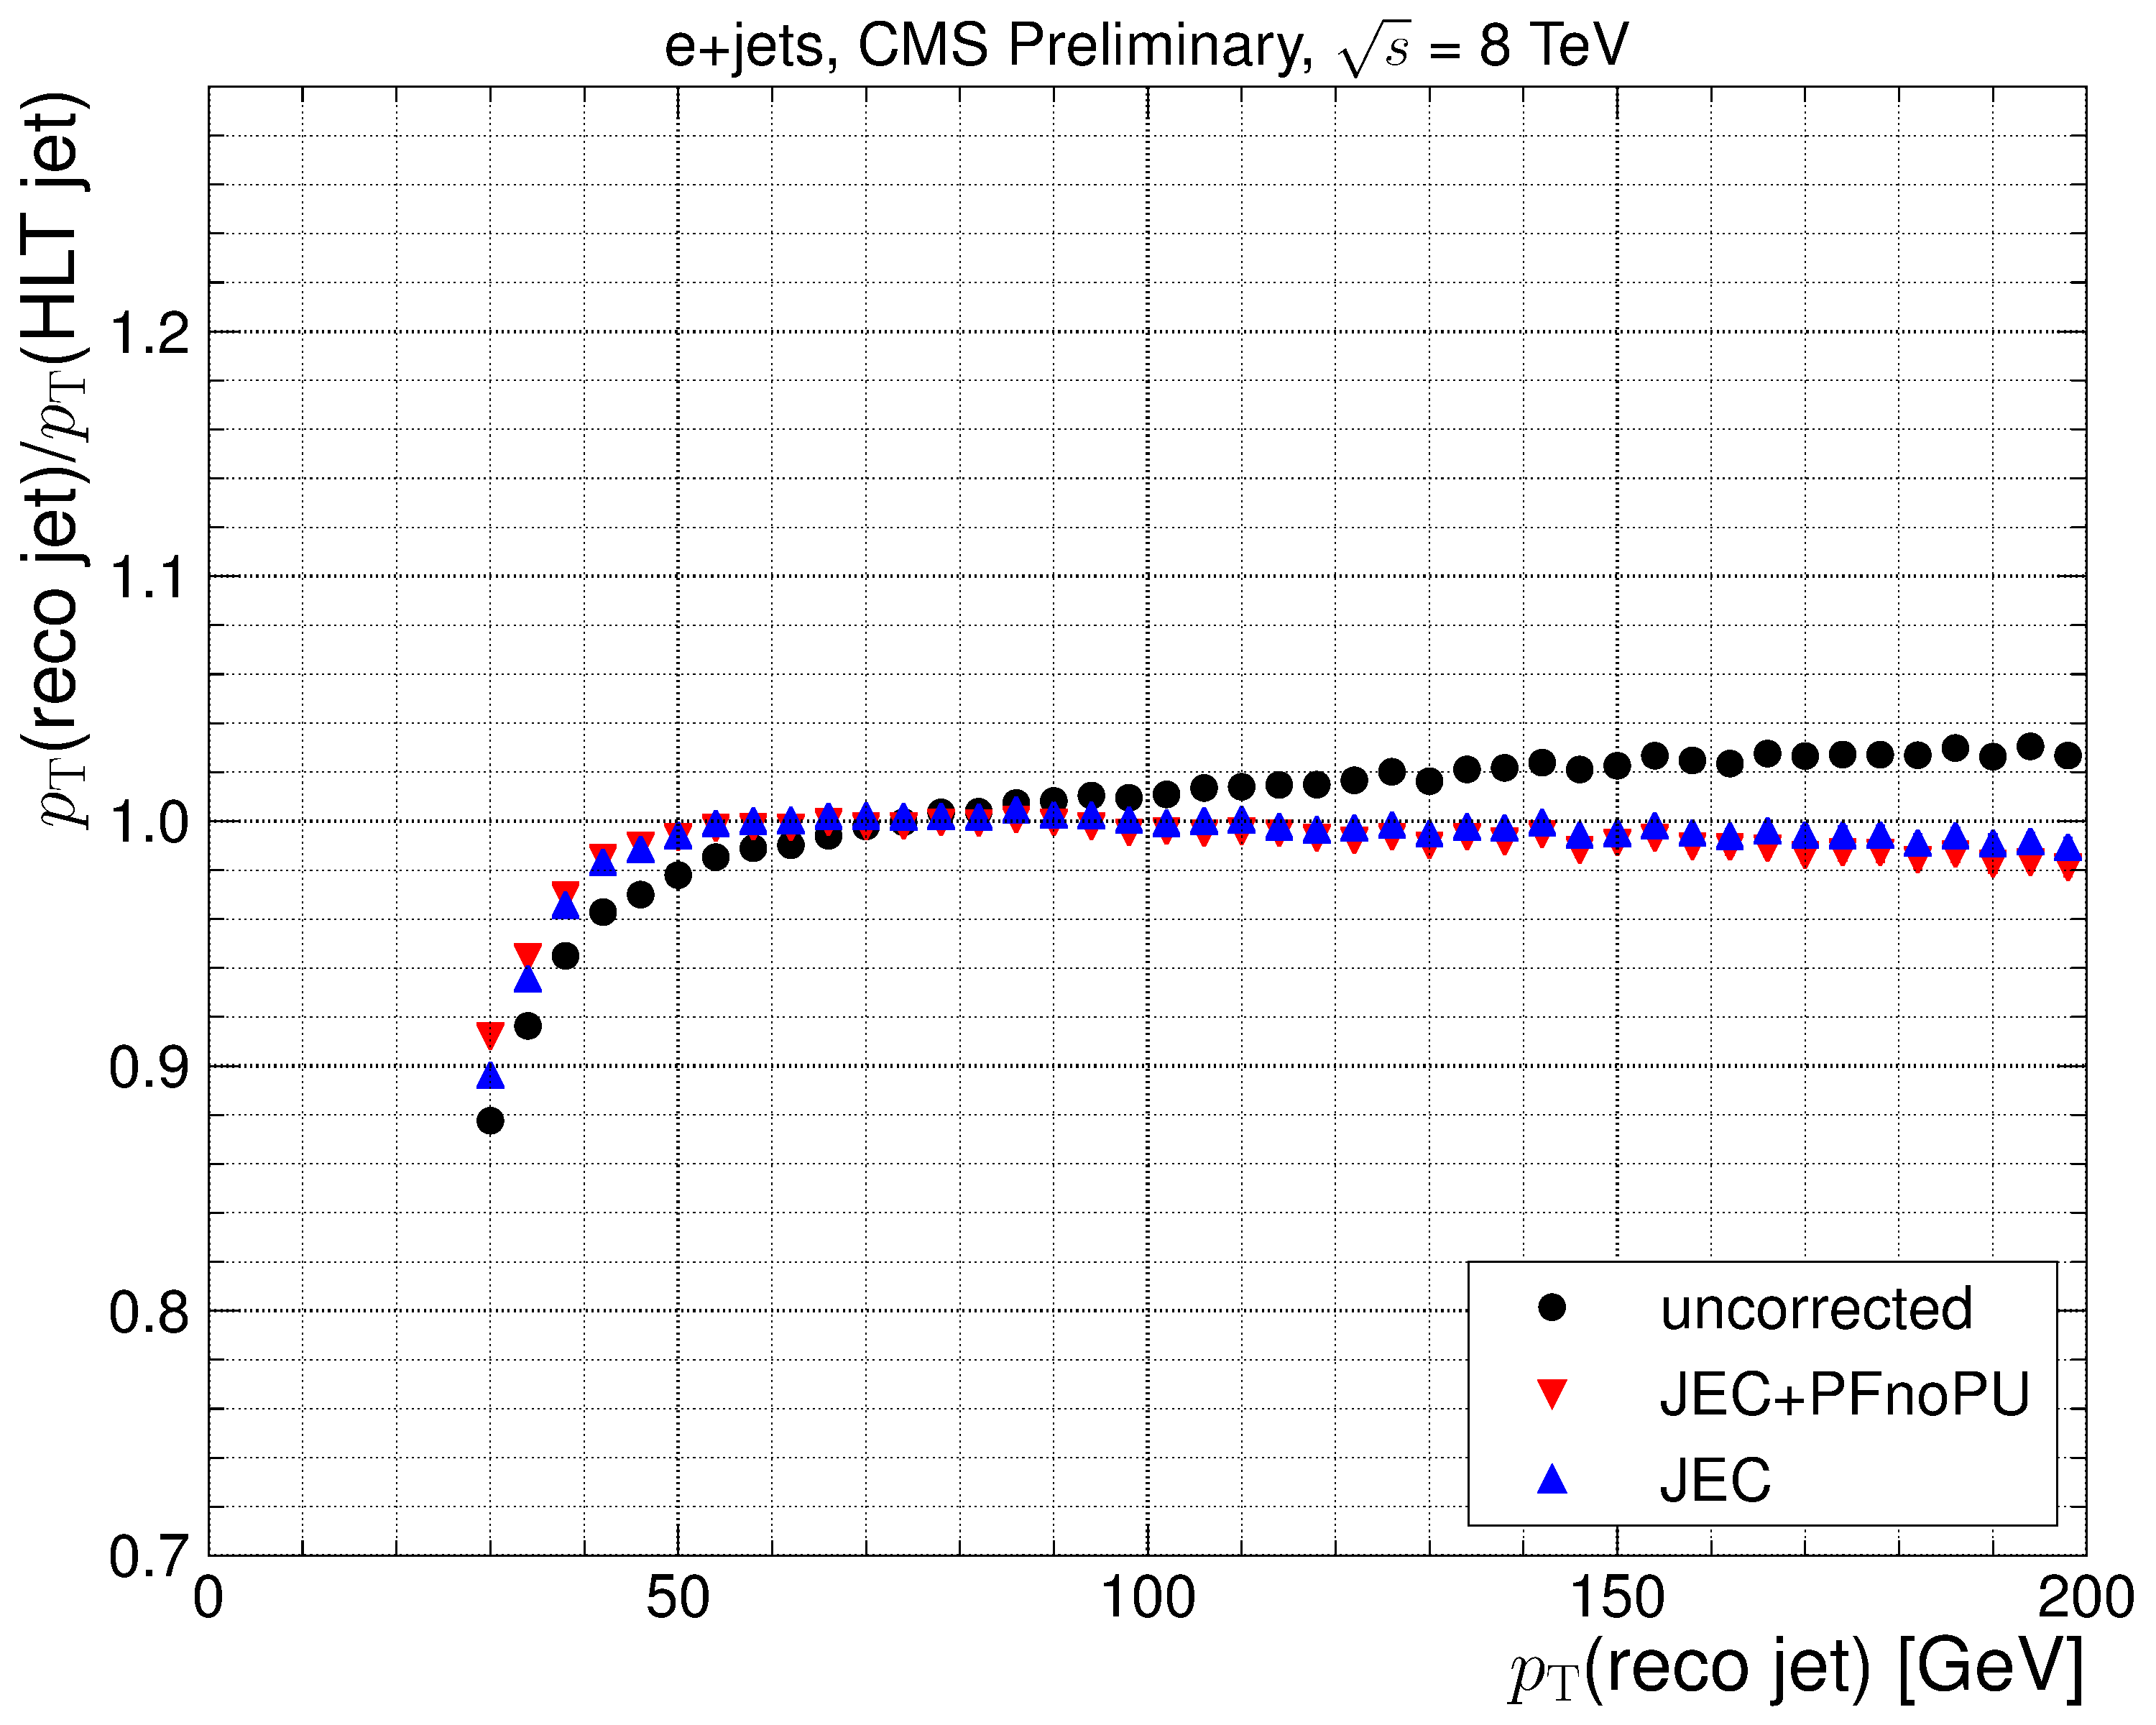
\includegraphics[width=0.5\textwidth]{ptRatio_pt_prof_comparison_correction_levels.pdf}}
  \hfill
  \subfloat[]{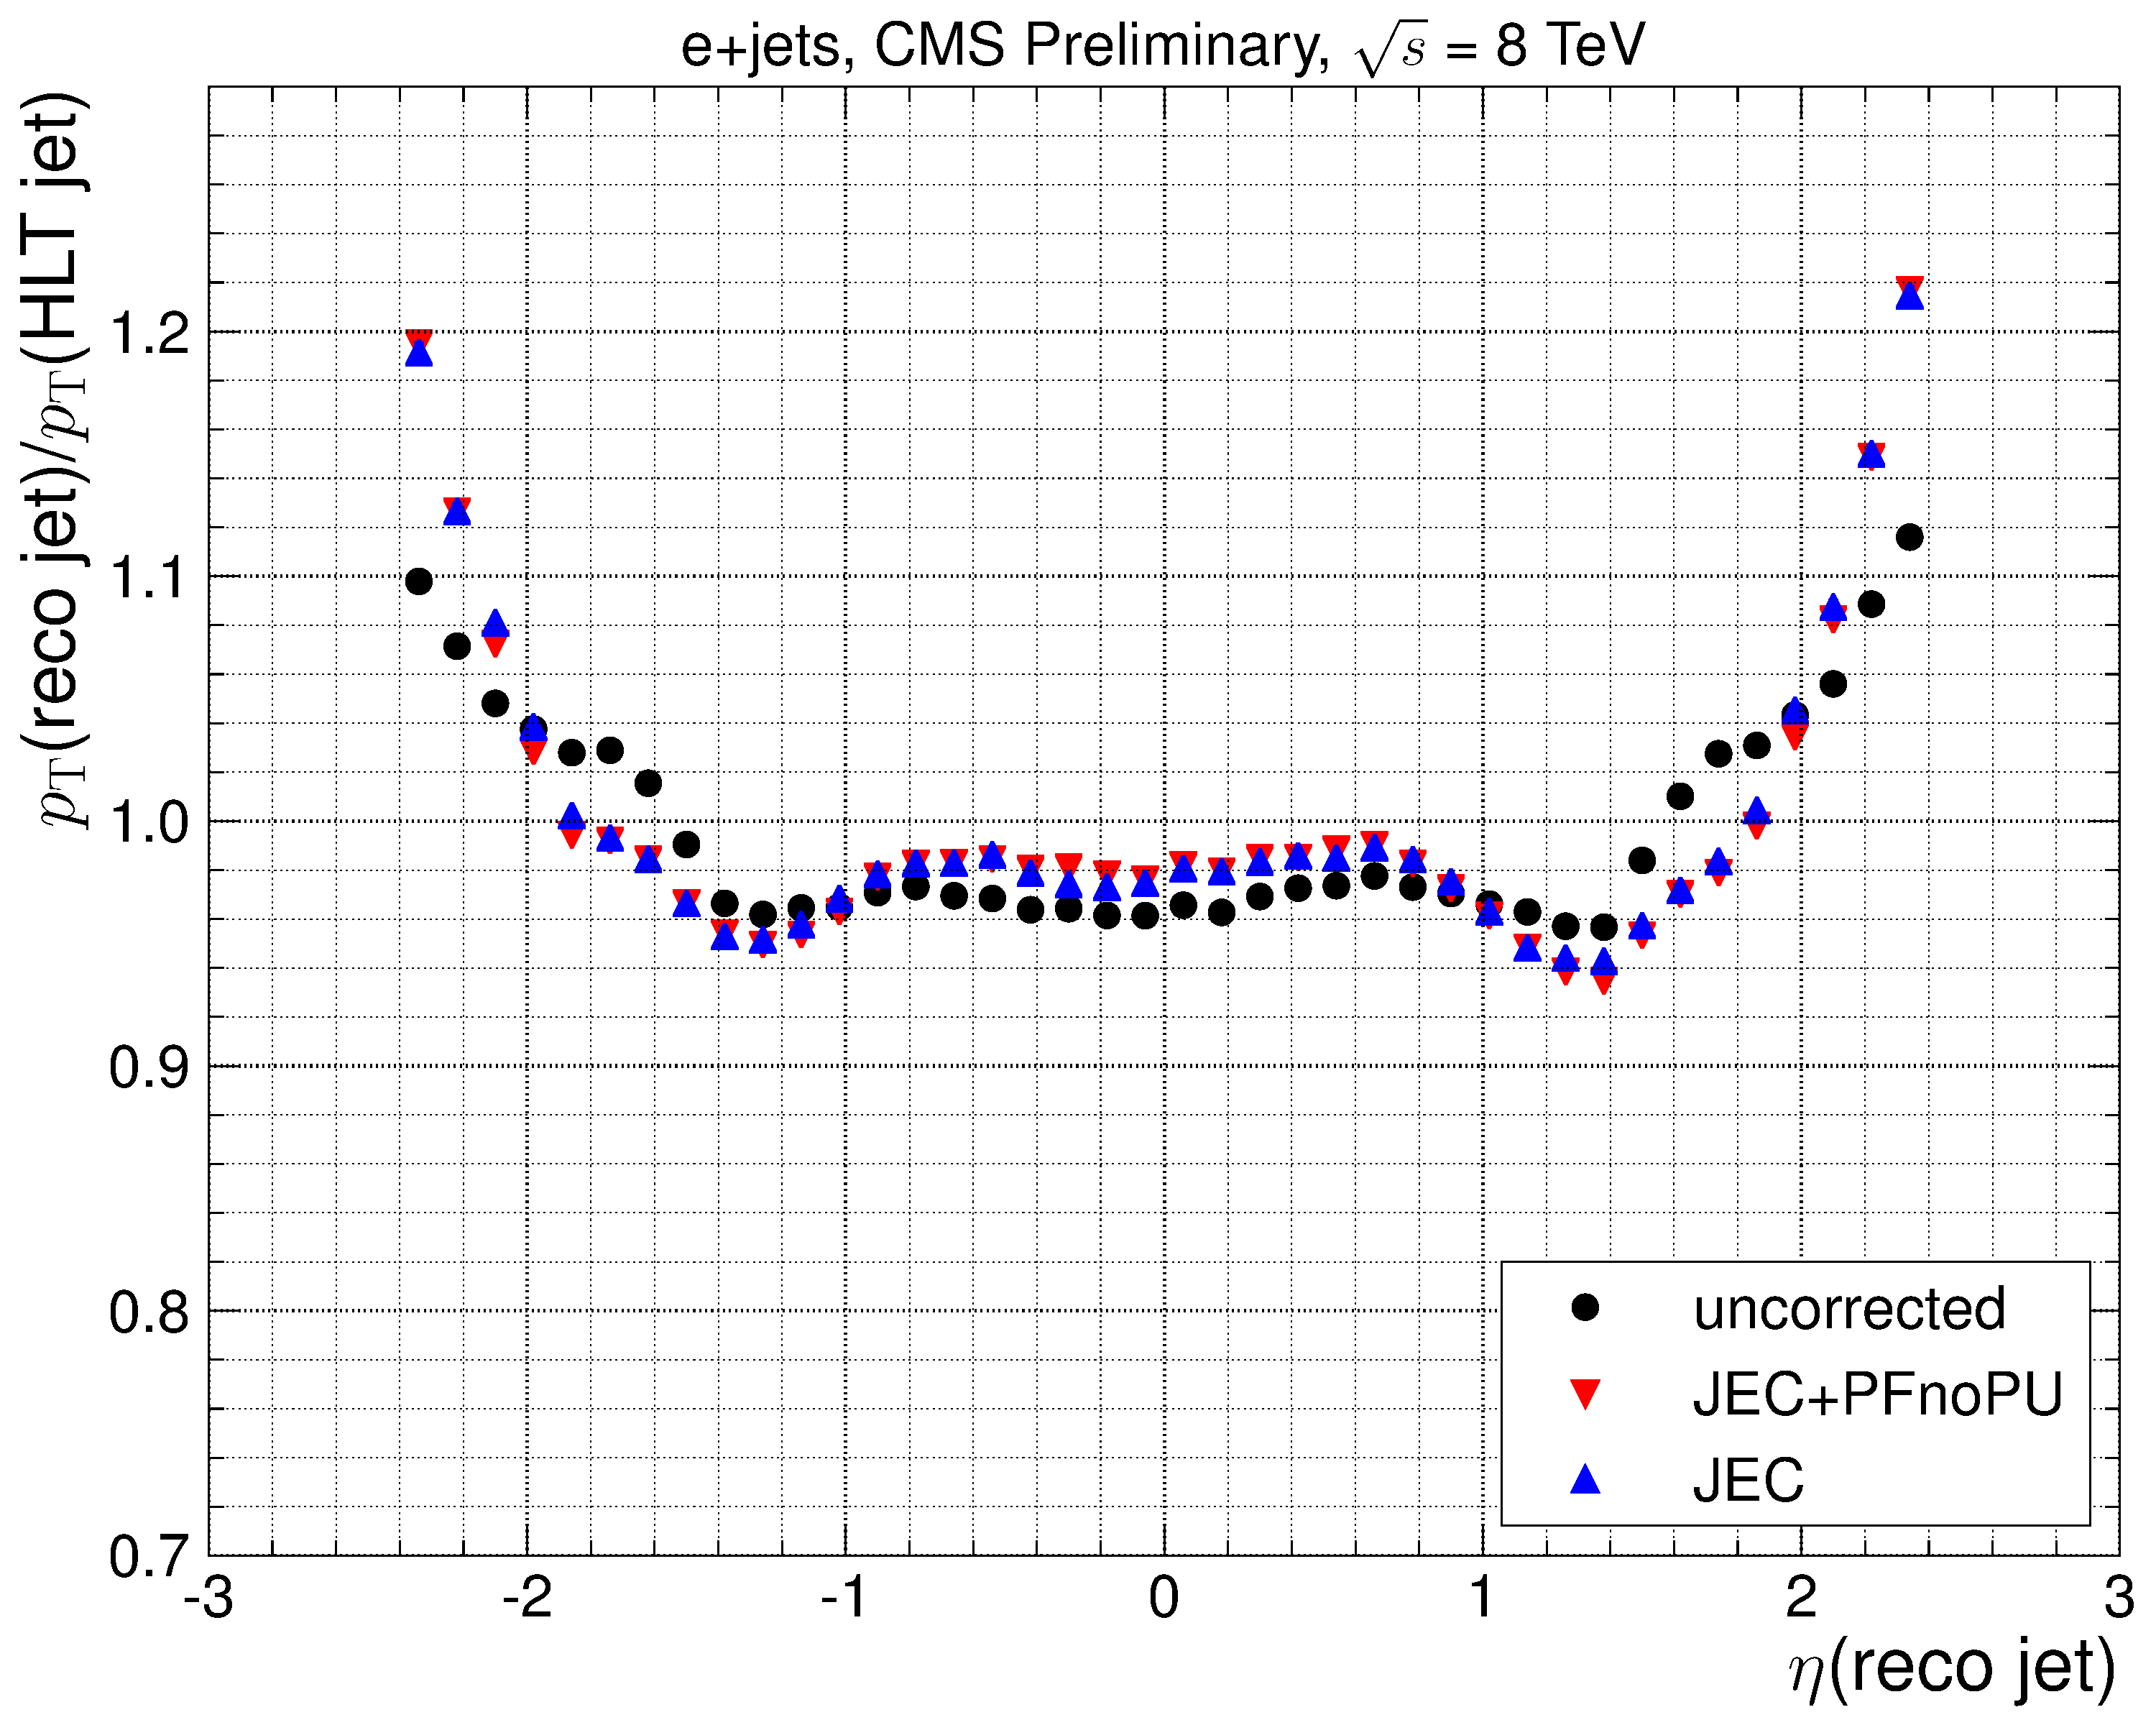
\includegraphics[width=0.5\textwidth]{ptRatio_eta_prof_comparison_correction_levels.pdf}} \\
  \subfloat[]{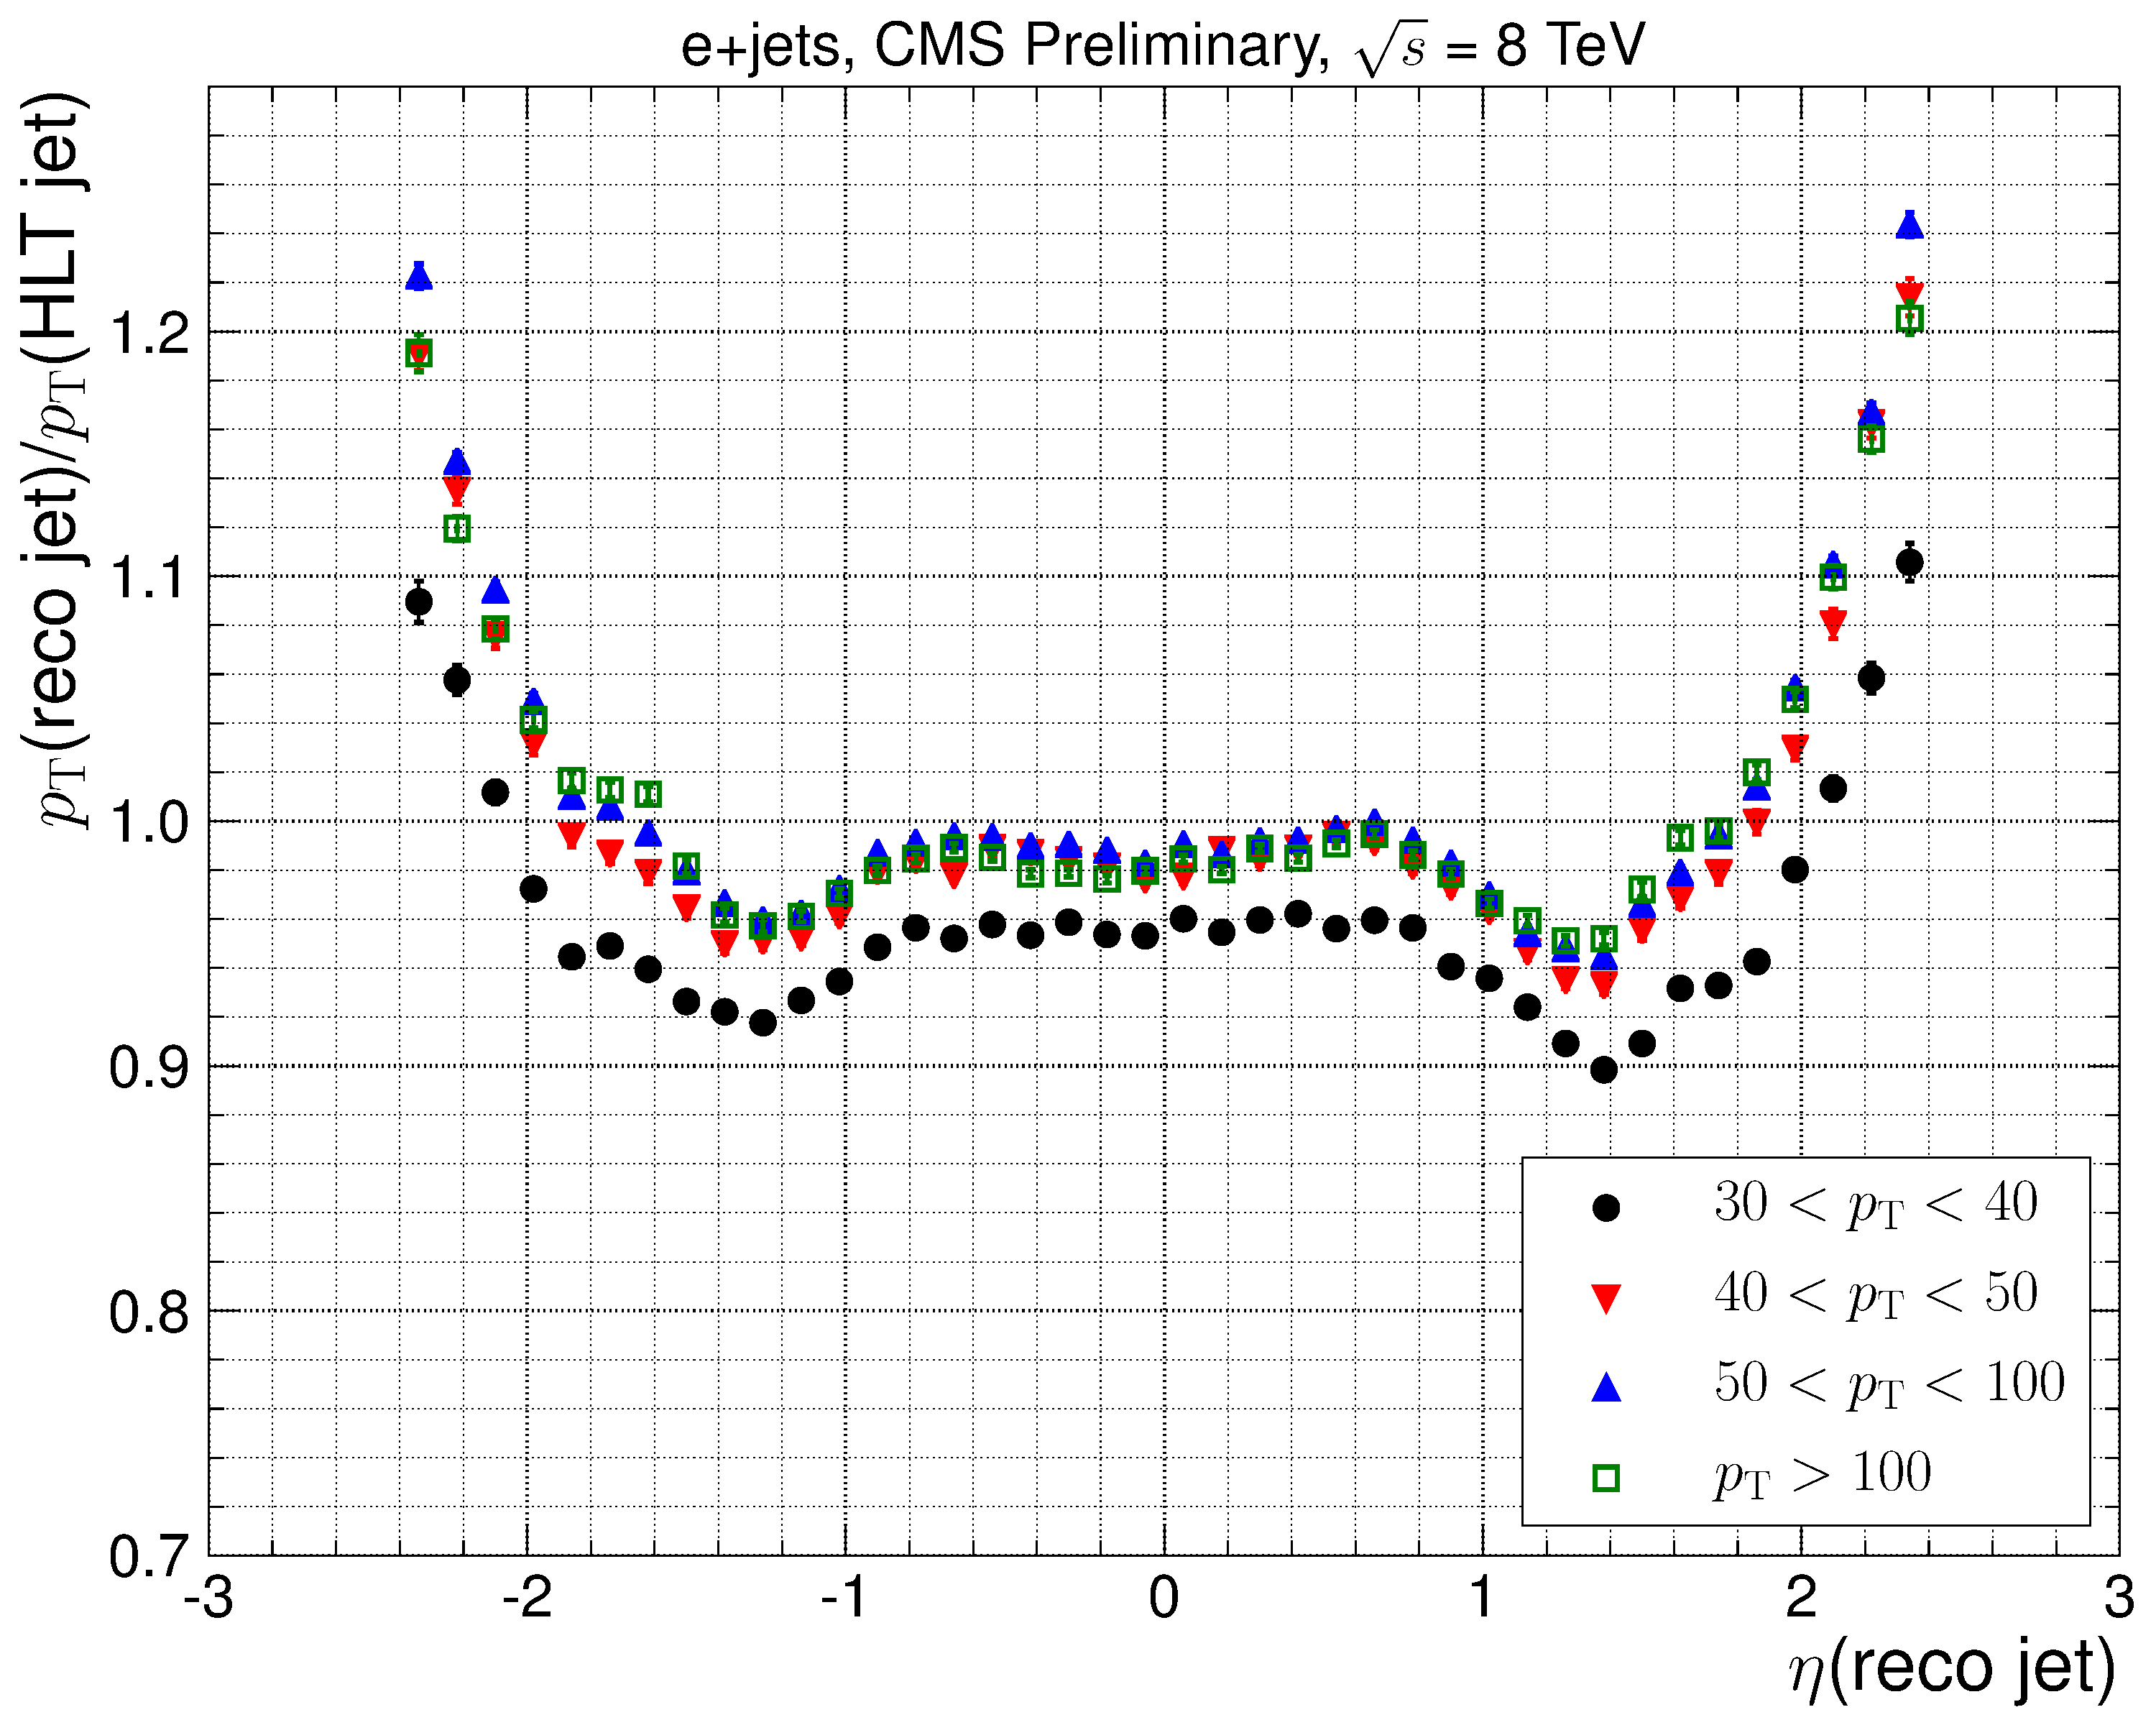
\includegraphics[width=0.88\textwidth]{ptRatio_eta_prof_comparison_pt_bins.pdf}}
  \caption[Jet response as a function of jet \pt and $\eta$]{Ratio of matched offline and online reconstructed jet
transverse momenta as a function of offline jet \pt (a) and $\eta$ (b) for different jet corrections and in slices of
offline jet \pt (c).}
\label{fig:top_hlt_jet_response} 
\end{figure}

Shorty after these results were presented to the trigger coordination, they were confirmed independently by other
experts within the JetMET group. Because of the time constraints associated with the luminosity increase schedule, a
following workaround solution was suggested. In order to re-gain the trigger efficiency, the threshold for the third jet
was dropped from \SI{30}{\GeV} to \SI{20}{\GeV}, which allowed application of jet energy corrections and charged hadron
subtraction with a minimum loss in the efficiency in the endcap region.

At the time of writing this thesis, the source of inadequacy of the jet response in the endcap region remains not fully
understood. One of the possible explanations is based on the observation that the number of fake tracks reconstructed
online is substantially larger than that in the offline reconstruction, which can potentially bias the PF jet
reconstruction on the HLT level. However, a full solution to this problem (and therefore derivation of adequate jet
energy corrections for online application) is still being sought for by a relevant group of experts.

\newpage
\section{Summary}
This chapter covered the service work performed by the author for the CMS collaboration, namely development, validation
and maintenance of high-level triggers for top quark physics, specifically for the electron channel of semileptonic
\ttbar decay signature. The importance and typical challenges of trigger development have been discussed. The modular
structure of high level triggers has been described in detail for electron plus jets trigger paths. A core of author's
contribution: the investigation of the effect of jet energy corrections applied on the HLT level to top trigger paths
has been presented, showing how it affects trigger efficiency and jet response distributions. An impact of charged
hadron subtraction applied online has also been studied and demonstrated.

% ------------------------------------------------------------------------


%%% Local Variables: 
%%% mode: latex
%%% TeX-master: "../thesis"
%%% End: 
